\documentclass[12pt,letterpaper,twoside]{article}
% Essential packages for technical documentation
\usepackage[margin=1in]{geometry}  % Page margins
\usepackage{amsmath,amssymb,amsfonts}  % Advanced math formatting
\usepackage{mathtools}  % Extension to amsmath
\usepackage{bm}  % Bold math symbols
\usepackage{graphicx}  % For images
\usepackage{booktabs}  % Professional tables
\usepackage{array}  % Extended table features
\usepackage{multirow}  % Multi-row cells in tables
\usepackage[shortlabels]{enumitem}  % Customized lists
\usepackage{fancyhdr}  % Custom headers and footers
\usepackage{titlesec}  % Custom section formatting
\usepackage{hyperref}  % Hyperlinks
\usepackage{listings}  % Code listings
\usepackage{color}  % Text colors
\usepackage[table]{xcolor}  % Extended color support
\usepackage{microtype}  % Typography improvements
\usepackage{placeins} % FloatBarrier
\usepackage{chngcntr} % counterwithin

% Point table references at top of table while keeping caption below
\usepackage[tableposition=bottom]{caption}

\usepackage{mathptmx}  % Times Roman font with math support

\newcommand{\doctitle}{Cinepak for Jaguar}
\newcommand{\doccopy}{© 1995 Radius Inc. \& Atari Corp.}
\newcommand{\docdate}{16 June, 1995}
\newcommand{\titformat}[1]{{\textbf{\textit{#1}}}}
\newcommand{\headerformat}[1]{{\footnotesize\titformat{#1}}}

% Page setup
\setlength{\parindent}{0pt}     % Remove paragraph indentation
\setlength{\parskip}{1em}       % Add vertical space between paragraphs
\setlength{\headheight}{15pt}	% Shut fancy head warnings up
\pagestyle{fancy}
\fancyhf{}  % Clear header/footer
\fancyhead[LO]{\headerformat{\doctitle}}
\fancyhead[RE]{\headerformat{\doctitle}}
\fancyhead[LE]{\headerformat{Page \thepage}}
\fancyhead[RO]{\headerformat{Page \thepage}}
\fancyfoot[LO]{\headerformat{\doccopy}}
\fancyfoot[RE]{\headerformat{\doccopy}}
\fancyfoot[LE]{\headerformat{\docdate}}
\fancyfoot[RO]{\headerformat{\docdate}}
\fancyfoot[CO]{\headerformat{Confidential \raisebox{-1pt}{
\includegraphics[height=8pt]{aux/atari_jaguar_logo.pdf}} Information}}
\fancyfoot[CE]{\headerformat{Property of \raisebox{-1pt}{
\includegraphics[height=8pt]{aux/atari_jaguar_logo.pdf}} Atari Corporation}}
\renewcommand{\headrulewidth}{0.4pt}
\renewcommand{\footrulewidth}{0.4pt}

% Title formatting
\titleformat{\section}[block]
  {\normalfont\Large\bfseries}
  {}
  {0pt}
  {\colorsection}

\titleformat{\subsection}[block]
  {\normalfont\large\bfseries}
  {}
  {0pt}
  {\colorsubsection}

\titleformat{\subsubsection}[block]
  {\normalfont\bfseries}
  {}
  {0pt}
  {\colorsubsubsection}

\newcommand{\colorsection}[1]{%
  \colorbox{lightgray}{\parbox{\dimexpr\columnwidth-2\fboxsep-2\fboxrule\relax}{\strut\thesection~#1\strut}}}

\newcommand{\colorsubsection}[1]{%
  \colorbox{lightgray}{\parbox{\dimexpr\columnwidth-2\fboxsep-2\fboxrule\relax}{\strut\thesubsection~#1\strut}}}

\newcommand{\colorsubsubsection}[1]{%
  \colorbox{lightgray}{\parbox{\dimexpr\columnwidth-2\fboxsep-2\fboxrule\relax}{\strut\thesubsubsection~#1\strut}}}

% Custom environments for special boxes or notes
\newenvironment{technote}
  {\begin{center}\begin{itshape}\begin{tabular}{|p{0.9\textwidth}|}
   \hline\\}
  {\\\\
   \hline
   \end{tabular}\end{itshape}\end{center}}

% Make table counters reset for each section
\counterwithin{table}{section}
\captionsetup[table]{labelfont=bf,labelsep=endash}

\counterwithin{figure}{section}
\captionsetup[figure]{labelfont=bf,labelsep=endash}
\renewcommand\thefigure{\arabic{section}-\Alph{figure}}

% Add a command to format the text in table header rows
\newcommand{\tabheadtxt}[1]{\multicolumn{1}{c}{\textcolor{white}{\textbf{#1}}}}

% Document info
\title{\Huge{\textbf{\doctitle}}\\ \vspace{0.5cm} \Large{Technical Documentation}}
\author{Converted from Original Document}
\date{\today}

\begin{document}

\maketitle
\thispagestyle{empty}  % No page number on title page

\tableofcontents
\newpage

\section{Introduction}
This documents describes \titformat{\doctitle}, a combination of utilities and code that has been developed to enable creation of high-quality video material which can be played back from the Jaguar CD-ROM. Playback rates of 30 frames per second are possible even with full-screen (320x200), 16-bit per pixel images. In fact, even higher resolutions and/or frame rates are possible provided the overall data rate is reasonable.

The \titformat{\doctitle} package is based upon Radius' proprietary Cinepak video compression technology\footnote{Cinepak is a trademark of Radius Inc.}, which was specifically developed for this type of application; it consists of the following main elements:

\begin{enumerate}[left=0pt .. 36pt]
\item Interface definition and linkable object code for the Cinepak decompressor.
\item Definition of a file format which interleaves audio and video in a manner suitable for playback on Jaguar, together with sample playback code which illustrates how to manage the periodic access to the CD-ROM and maintain synchronization between audio and video.
\item A utility to convert Cinepak-encoded QuickTime movies to the Jaguar Cinepak film format and perform necessary manipulations prior to recording on CD-ROM.
\item Three sample Jaguar films on CD-ROM.
\end{enumerate}

The Cinepak decompressor and the interface to it are discussed in the \textbf{Cinepak Decompressor} section. The Jaguar film format is discussed in the \textbf{Jaguar Film Format} section. The details of the sample player code are described in the \textbf{Sample Playback Code} section. The use of the film conversion utility is discussed in the \textbf{Jaguar Cinepak Utility For Macintosh} section. The content of a sample Jaguar CD-ROM containing Cinepak films is briefly described in the \textbf{Sample Jaguar Films} section. The layout of film data on a CD-ROM is discussed in the \textbf{Using A Jaguar Cinepak Film With CD-ROM} section.

\section{Cinepak Decompressor}
In this section, we define the interface to the two code modules and briefly describe the operation of the flags. For an example of how these elements are incorporated in playing a Jaguar film, see the \textbf{Sample Playback Code} section.

\subsection{68000 Module}
The \texttt{codec.o} module consists of approximately 700 bytes of 68000 code. There are three user callable functions, \texttt{CheckKeyFrame}, \texttt{PreDecompress}, and \texttt{Decompress}. The interfaces to these routines is specified below. All the routines preserve all 68000 registers. All parameters used by these routines are passed on the stack. The return value is also returned on the stack. Cleaning up the stack upon return from any of these three routines is the responsibility of the calling program.

\subsubsection{CheckKeyFrame()}
This routine is called to determine whether or not the current frame is a key frame.\footnote{Cinepak generally relies upon frame differencing to compress video data; however, the encoder periodically inserts a key frame into the data stream. Such a frame can be decompressed without reference to any frames which precede it. A key frame may either occur naturally as a result of an abrupt change of scene, or can be injected into the data stream at a prescribed rate to aid random access or resynchronization with audio.}

\begin{table}[h]
\centering
\begin{tabular}{|c|c|p{8cm}|}
\hline
\rowcolor{black}
\tabheadtxt{Stack Offset} & \tabheadtxt{Size} & \tabheadtxt{Description} \\
\hline
4(a7) & 4 & Return value. Must be set to 0 prior to entry. Will be set to 1 upon exit if key frame is detected. \\
\hline
(a7) & 4 & Address of start of frame. \\
\hline
\end{tabular}
\caption{68000 stack setup before call to CheckKeyFrame.}
\label{tab:checkKeyFrame}
\end{table}
\FloatBarrier

\subsubsection{PreDecompress()}
This routine is called to set up the tables needed to draw pixels on the display.

\begin{table}[h]
\centering
\begin{tabular}{|c|c|p{12cm}|}
\hline
\rowcolor{black}
\tabheadtxt{Stack Offset} & \tabheadtxt{Size} & \tabheadtxt{Description} \\
\hline
10(a7) & 4 & Return value. Value prior to entry is not important. 0 = returned upon successful completion non-zero Error occurred. \\
\hline
6(a7) & 4 & Address of \$3000 byte auxiliary Cinepak data buffer (see section 2.4) \\
\hline
2(a7) & 4 & Address of start of frame in Cinepak bitstream. \\
\hline
(a7) & 2 & Flag which indicates video data type:
	\begin{itemize}[nosep]
	\item[] 0 = Cinepak compressed-RGB format
	\item[] 1 = Atari CRY format or expanded RGB
	\end{itemize}\\
\hline
\end{tabular}
\caption{68000 stack setup before call to PreDecompress.}
\label{tab:predecompress}
\end{table}
\FloatBarrier

\subsubsection{Decompress()}
This is the routine that actually displays the pixels.

\begin{table}[h]
\centering
\begin{tabular}{|c|c|p{10cm}|}
\hline
\rowcolor{black}
\tabheadtxt{Stack Offset} & \tabheadtxt{Size} & \tabheadtxt{Description} \\
\hline
16(a7) & 4 & Value prior to entry is not important. Returns:
	\begin{itemize}[nosep]
	\item[] 0 = successful completion
	\item[] non-zero = error
	\end{itemize}\\
\hline
12(a7) & 4 & Address of \$3000 byte auxiliary Cinepak data buffer (see section 2.4) \\
\hline
8(a7) & 4 & Address of start of frame in bitstream. \\
\hline
4(a7) & 4 & Frame buffer address of top left corner of image. \\
\hline
2(a7) & 2 & Bytes per row in frame buffer \\
\hline
(a7) & 2 & Phrase Interleave Factor \\
\hline
\end{tabular}
\caption{68000 stack setup before call to Decompress.}
\label{tab:decompress}
\end{table}
\FloatBarrier

The latest version of Cinepak for Jaguar supports phrase interleaving for faster double or triple buffering schemes. If zero is passed as the phrase interleave factor, Cinepak will perform normally, writing its data contiguously in memory. A phrase interleaving factor of one will cause one phrase to be skipped for every one written. A phrase interleaving factor of two will cause two phrases to be skipped for every one written, and so on. This is done in a way that is compatible with similar features in the Object Processor and Blitter. By interleaving the buffers which must be blitted back and forth, the frequency of DRAM page faults drops significantly, increasing the available bus bandwidth.

\subsubsection{HaltCPK()}
This routine shuts down the Cinepak decompression code running in the GPU at the end of the current frame. It takes no parameters. To restart Cinepak you must start from the beginning again.

\subsection{GPU Module}
The \texttt{gpucode.og} module consists of approximately 2200 bytes of relocatable GPU code. The labels \texttt{DECOMP\_S} and \texttt{DECOMP\_E} defined in the \texttt{gpucode.og} module are used to locate the beginning and end of the Cinepak GPU code so that it may be copied to the GPU's internal RAM for execution.

After the code has been copied over to internal GPU RAM, the GPU is started. The GPU code detects the address at which it has been loaded by looking at the \texttt{GPUOffset} variable and then patches all instructions and table values which are position-dependent. It then notifies the 68000 via the \texttt{GPU\_READY} flag (see Section 2.3) that it is ready to perform decompression tasks.

The Cinepak GPU code may be run from either register bank with some limitations. By default, Cinepak assumes it will run from Bank \#0 and will set R31 to point to ten longwords of interrupt stack that it provides. As Cinepak requires registers R0-R27 (and R28-R31 are reserved for interrupts), if you run Cinepak in Bank \#0, any interrupt code must preserve all Bank \#0 registers. To run Cinepak in Bank \#1 you must perform the following steps:

\begin{enumerate}[nosep, left=0pt .. 36pt]
\item Load the Cinepak GPU code into GPU RAM.
\item Load a small startup stub somewhere else in GPU RAM.
\item Have the startup stub provide interrupt stack space and store the location in R31.
\item Switch to the second register bank.
\item Using the information in \texttt{GPU\_OFFSET}, jump to the head of the Cinepak code.
\end{enumerate}

When these above steps are performed, Cinepak will harmlessly change R31 in Bank \#1 and continue to run from Bank \#1. Interrupts (which must run in Bank \#0) may then use R0-R27 of Bank \#0 without saving them.

Once the system has been initialized, all GPU functions are invoked from within the routines in the \texttt{codec.o} module; no attempt should ever be made by your code to directly access the GPU decompression functions.

While the GPU is executing decompression functions, the 68000 is halted (a \texttt{stop \#\$2000} instruction is executed within \texttt{codec.o}). When the GPU finishes its task, it interrupts the 68000; the interrupt service routine sets a semaphore which is polled within \texttt{codec.o} to reawaken the 68000. This mechanism provides a 5-10\% improvement in performance by minimizing GPU/68000 bus contention, and should not be circumvented.

The sample player program includes a utility subroutine named \texttt{LoadGPU} in the \texttt{util.s} file. This routine copies the GPU code from \texttt{gpucode.og} into GPU memory (see section 5.5). The load address is offset from the base of GPU memory by the constant value \texttt{GPU\_OFFSET}, defined in the application-specific \texttt{CINEPAK.INC} include file. This offset is necessary to avoid collision with the GPU interrupt vectors.

Sample code for the GPU startup sequence appears in the module \texttt{player.s} (see Section 5), in the vicinity of label \texttt{WaitGPU}.

\subsection{Flags}
Storage for two flag variables must be declared within the DRAM address space. These are defined in Table \ref{tab:dramflags}. The initial values of these flags are not important.

\begin{table}[h]
\centering
\begin{tabular}{|c|c|p{12cm}|}
\hline
\rowcolor{black}
\tabheadtxt{Flag} & \tabheadtxt{Size} & \tabheadtxt{Description} \\
\hline
semaphore & 2 & Cleared within \texttt{codec.o} upon invocation of GPU task. Set by interrupt service routine upon completion of GPU task. \\
\hline
GPUOffset & 4 & Relocation offset of GPU code. Before you execute the GPU code from \texttt{gpucode.og}, this variable must be set to the offset from the beginning of GPU internal RAM (G\_RAM) where the GPU code has been loaded.\newline
\newline
The sample player program sets this to the constant value \texttt{GPU\_OFFSET} at time GPU code is loaded.\\
\hline
\end{tabular}
\caption{Flags declared in DRAM address space.}
\label{tab:dramflags}
\end{table}
\FloatBarrier

An additional flag is declared (internal to \texttt{gpucode.og}) within GPU internal address space and must be accessed by the 68000, as defined in Table \ref{tab:gpuflags}.

\begin{table}[h]
\centering
\begin{tabular}{|c|c|p{11cm}|}
\hline
\rowcolor{black}
\tabheadtxt{Flag} & \tabheadtxt{Size} & \tabheadtxt{Description} \\
\hline
GPU\_READY & 4 & Cleared by 68000 prior to GPU startup. Set by GPU when initialization procedure has been completed.\newline
\newline
To account for GPU code relocation, you must add the value of \texttt{GPUOffset} to this symbol in order to get the correct address. (For an example, see the code immediately before the \texttt{WaitForGPU} label in the sample program's \texttt{player.s} source file.) \\
\hline
\end{tabular}
\caption{Flag declared in GPU internal address space.}
\label{tab:gpuflags}
\end{table}
\FloatBarrier

\section{Jaguar Film Format}

The Cinepak bitstream is simply a source for a continuous stream of video; the bitstream contains no information pertaining to time, frame rate, or synchronization of video with other media such as audio. 

To provide a time reference and synchronization among different media, the Cinepak bitstream must be embedded in some higher-level structure that is aware of time and the existence of media other than video. The Jaguar film format has been devised to meet these requirements. 

The Jaguar film format exists in two flavors: 

\begin{enumerate}[1), left=0pt .. 36pt]
\item Smooth. This format is useful for playback of multiple low-resolution (for example, less than 160x100) films or a single film of higher resolution, provided in either case that the duration is very short (usually 3 or 4 seconds maximum). In this case, all the film data could be stored and played from ROM, or could be retrieved from the CD-ROM in a single brief access and loaded into DRAM for playing.
\item Chunky. This format is designed for playback of longer films that cannot fit in DRAM all at once. Here, periodic access to the CD-ROM is required on a continuing basis, so some mechanism must be incorporated in the film structure for locating and identifying the film data that are needed for display at a particular time.
\end{enumerate}

The film formats are described in detail in the sections 3.1 and 3.2.

Atari's existing sample Cinepak player code only knows how to play Chunky-format Cinepak Films. If your program needs to play smooth films, the changes would needed would be minor. 

\subsection{Smooth Format}

Table \ref{tab:smoothfmt} defines the structure of a smooth film at the highest level. 

\begin{table}[h]
\centering
\begin{tabular}{|c|c|p{10cm}|}
\hline
\rowcolor{black}
\tabheadtxt{Field} & \tabheadtxt{Size} & \tabheadtxt{Description} \\
\hline
Frame Header & 16 & Global film header\\
\hline
Frame Description & 20 & Frame size and compression type\\
\hline
Audio Description & 20 & Audio data format description\\
\hline
Sample Table & 16 + (n * 16) & Index to film samples which follow; n is number of samples\\
\hline
Film Samples & variable & Audio blocks and video frames\\
\hline
\end{tabular}
\caption{Smooth film format.}
\label{tab:smoothfmt}
\end{table}
\FloatBarrier

The frame header identifies the ensuing data as a Jaguar film and gives the offset to the start of the film data; its structure is defined in Table \ref{tab:framehead}. The frame description provides information about pixel resolution and the format of the compressed video; Table \ref{tab:framedesc} describes this structure. The audio description contains information about the format of any audio data included in the film. This is discussed in Table \ref{tab:audiodesc}. (Note that some older Jaguar Cinepak films may not include this field.) The sample table provides a time-based index to the ensuing audio and video data which form the actual content of the film; Table \ref{tab:sampletab} defines the structure of the sample table.

At the film sample level, the data stream is interleaved blocks of audio and video sample information; the time field of the sample record holds the key to the multiplexing scheme (see discussion following Table \ref{tab:samplerec}). The audio data itself uses the format defined by the film's audio description atom. The video data stream is in the proprietary Cinepak format, which is interpreted by the Cinepak decompressor.

\subsubsection{Frame Header}

\begin{table}[h]
\centering
\begin{tabular}{|c|c|p{10cm}|}
\hline
\rowcolor{black}
\tabheadtxt{Field} & \tabheadtxt{Size} & \tabheadtxt{Description} \\
\hline
Header & 4 & Human readable tag: 'FILM'\\
\hline
AtomSize & 4 & Size of film header, plus ensuing frame description and sample table\\
\hline
Version & 4 & Not used\\
\hline
Reserved & 4 & Not used\\
\hline
\end{tabular}
\caption{Structure of frame header.}
\label{tab:framehead}
\end{table}
\FloatBarrier

The frame header is a 16-byte structure comprised of four long-word fields. The Header field is a human-readable tag, 'FILM', which identifies the ensuing global data structure as a Jaguar film. The AtomSize field gives the offset in bytes from the start of the header to the beginning of the audio and video data records; this offset includes the size of the frame header itself, plus the sizes of the ensuing frame description and sample table structures. The Version and Reserved fields are not currently used; developers are free to use these as they wish.

\subsubsection{Frame Description Atom}

\begin{table}[h]
\centering
\begin{tabular}{|c|c|p{10cm}|}
\hline
\rowcolor{black}
\tabheadtxt{Field} & \tabheadtxt{Size} & \tabheadtxt{Description} \\
\hline
Header & 4 & Human readable tag: 'FDSC'\\
\hline
AtomSize & 4 & Size of frame description atom (=20)\\
\hline
CType & 4 & Human readable compression type:
\newline
	\begin{itemize}[nosep]
	\item[] 'cvid' = Cinepak compressed-RGB format
	\item[] '\$CRY' = Expanded Atari CRY format
	\item[] '\$RGB = Expanded RGB format
	\end{itemize}\\
\hline
Height & 4 & Number of display lines\\
\hline
Width & 4 & Number of pixels per line\\
\hline
\end{tabular}
\caption{Structure of frame description atom.}
\label{tab:framedesc}
\end{table}
\FloatBarrier

The frame description is a 20-byte structure comprised of five long-word fields. The Header field is a human-readable tag, 'FDSC', which identifies the structure as a frame description. The AtomSize field contains the size of the frame description atom (i.e. 20 bytes). The CType field contains a human-readable code which identifies the format of the compressed video; two modes are recognized: 

\begin{table}[h]
\centering
\begin{tabular}{|c|p{7cm}|}
\hline
\rowcolor{black}
\tabheadtxt{Value} & \tabheadtxt{Meaning} \\
\hline
'cvid' & Cinepak compressed-RGB format\\
\hline
'\$CRY' & Cinepak Expanded Atari CRY format\\
\hline
'\$RGB & Cinepak Expanded RGB format\\
\hline
\end{tabular}
\caption{Frame Description Atom CType values}
\label{tab:ctypevals}
\end{table}
\FloatBarrier

The Height and Width fields specify the vertical and horizontal resolution of the video in pixels. 

\subsubsection{Audio Description Atom}

\begin{table}[h]
\centering
\begin{tabular}{|c|c|p{8cm}|}
\hline
\rowcolor{black}
\tabheadtxt{Field} & \tabheadtxt{Size} & \tabheadtxt{Description} \\
\hline
Header & 4 & Human readable tag: 'ADSC'\\
\hline
AtomSize & 4 & Size of audio description atom (=20)\\
\hline
AudioData & 4 & Audio Data Description\\
\hline
SCLK & 4 & SCLK timer value for audio playback\\
\hline
AudioDrift & 4 & Drift rate value used adjust audio sample rate\\
\hline
\end{tabular}
\caption{Structure of audio description atom.}
\label{tab:audiodesc}
\end{table}
\FloatBarrier

The audio description atom is a 20-byte structure that defines the format of the audio data contained in the Cinepak film so that it may be played back properly. The Header field is a human-readable tag 'ADSC' which identifies the structure as an audio description atom. The AtomSize field specifies the size of the structure (20 bytes).

The AudioData field is a bitmapped flag that defines the data format of the audio, i.e. mono or stereo, compressed or non-compressed, 8-bit samples or 16-bit samples, and so forth. See Table \ref{tab:audioflags} for a definition of the meanings of each bit. Note that the proper utilization of this information is the responsibility of the Cinepak player application. 

\begin{table}[h]
\centering
\begin{tabular}{|c|p{8cm}|}
\hline
\rowcolor{black}
\tabheadtxt{Bits} & \tabheadtxt{Meaning}\\
\hline
0 & 0 = Mono, 1 = Stereo\\
\hline
1 & 0 = 8-bit, 1 16-bit\\
\hline
2-7 & Audio Compression Type:
\newline
	\begin{itemize}[nosep]
	\item[] 0 = uncompressed
	\item[]	1 = n\textsuperscript{2} compression
	\item[] other values are reserved 
	\end{itemize}\\
\hline
8-30 & Reserved\\
\hline
31 & Two's Complement audio flag\\
\hline
\end{tabular}
\caption{Audio description flag bits}
\label{tab:audioflags}
\end{table}
\FloatBarrier

The SCLK field contains the value which should be used with the Jaguar's SCLK 
timer to set the DSP interrupt frequency for audio playback. In Jaguar Cinepak
films which have no audio information, the SCLK field will be set to $-1$
($\mathrm{FFFFFFFF}$).\footnote{This will only be true for films converted with versions of the Jaguar Cinepak Utilities dated June 1995 and later.}

The Audio Drift field specifies a 32-bit value that can be used by the player program's audio playback code to account for the difference between the audio data's original sample rate and the actual playback rate on the Jaguar. This value is added to an accumulator during each DSP sample rate interrupt. When a carry is generated, instead of proceeding to the next sample as usual, the current sample is reused instead. The audio drift rate is derived from the formula: 

\begin{equation}
\mathrm{DriftRate} = \frac{2^{32}}{\mathrm{SourceSampleRate} \div (\mathrm{SourceSampleRate} - \mathrm{JaguarSampleRate})}
\end{equation}

The Jaguar sample rate is determined by: 

\begin{equation}
\mathrm{VideoClockRate} = 26590906\,\mathrm{Hz} \text{ (NTSC)}, 26593900\,\mathrm{Hz} \text{ (PAL)} \\
\end{equation}
\begin{equation}
\mathrm{JaguarSampleRate} = \left\{\frac{\mathrm{VideoClockRate}}{2 \times (\mathrm{SCLK} + 1)} \div 32\right\}
\end{equation}

You can work backwards from the DriftRate value and the Jaguar Sample Rate to get the original sample rate. You might do this, for example, in the event that you wanted to change the DSP code to perform linear interpolation to adjust the playback sample rate, rather than simply repeating samples. The formula for this is:

\begin{equation}
\mathrm{SourceSampleRate} = \mathrm{JaguarSampleRate} + \frac{\mathrm{JaguarSampleRate}}{2^{32} \times \mathrm{DriftRate}}
\end{equation}

Note that older Jaguar Cinepak films may not contain an Audio Description Atom. If none is found, the player code should typically default to expecting 8-bit mono at a 22050 Hz (original) sample rate.

\subsubsection{Sample Table Atom}

\begin{table}[h]
\centering
\begin{tabular}{|c|c|p{10cm}|}
\hline
\rowcolor{black}
\tabheadtxt{Field} & \tabheadtxt{Size} & \tabheadtxt{Description} \\
\hline
Header& 4 & Human readable tag: 'STAB'\\
\hline
AtomSize & 4 & Size of sample table atom\\ 
\hline
Scale & 4 & Time scale of film\\ 
\hline
Count & 4 & Number of sample records in table\\
\hline
Sample records & 16 * Count & Array of sample records\\ 
\hline
\end{tabular}
\caption{Structure of sample table atom.}
\label{tab:sampletab}
\end{table}
\FloatBarrier

The sample table is a data structure which provides a time-based index to the film samples\footnote{The "sample" terminology is, unfortunately, somewhat ambiguous. In the context of a Cinepak film, it refers to a set of data which may be either audio or video. In the context of audio, it conventionally refers to the 8-bit or 16-bit datum which is read or written to a DAC. Where possibility for confusion exists, we use the terminology "block" to indicate the aggregate.}, i.e. blocks of audio and frames of video. The header is a human-readable tag, 'STAB', which identifies the structure as a sample table. The atom size field contains the size of the sample table atom, which encompasses the ensuing sample records. 

The scale field provides the time scale for the film, in fractional units of a second, i.e. the unit of time is the reciprocal of the scale. A value of 600 is commonly used in QuickTime movies, as it is the lowest common multiple of the common rates of 24, 25 and 30 frames per second. The MovieToFilm tool does not alter the time scale embedded in the QuickTime movie when a Jaguar film is created. 
The count field gives the number of sample records which immediately follow it; the sample record structure is defined in Table \ref{tab:samplerec}.

\subsubsection{Sample Record}

\begin{table}[h]
\centering
\begin{tabular}{|c|c|p{9cm}|}
\hline
\rowcolor{black}
\tabheadtxt{Field} & \tabheadtxt{Size} & \tabheadtxt{Description} \\
\hline
Start & 4 & Start of sample\\
\hline
Size & 4 & Number of bytes in sample\\
\hline
Time & 4 & Time at which to play sample\\
\hline
Duration & 4 & Duration of playback interval for sample\\
\hline
\end{tabular}
\caption{Structure of sample record.}
\label{tab:samplerec}
\end{table}
\FloatBarrier

The start field gives the starting address of the sample referenced by the sample record, relative to the end of the sample table. The end of the sample table coincides with the end of the frame header (see Table \ref{tab:framehead}). 

The size field gives the size of the referenced sample in bytes. Adding the start and size fields of the current sample record yields the value in the start field of the next sample record. 

The 31 least-significant bits in the time field of the sample record give the time at which the referenced sample is scheduled to be played, in the units specified by the scale field of the sample table. If the value is \$7FFFFFFF that indicates that the referenced sample (block) contains audio, not video, which should be played immediately following the end of the previous audio sample (block). 

The most significant bit of the time field indicates a shadow sync sample (0) or not (1); this is a carry- over from QuickTime that should be ignored by the sample player code.\footnote{For more information, see the book\textit{Inside Macintosh: QuickTime}, Addison-Wesley Publishing Company, 1993, pages. 2-134 to 2-135.}

The duration field of the sample record gives the play duration of the referenced sample, in units of the time scale. For an audio sample (block), the duration is meaningless; addition of the time and duration fields of the current video sample record yields the value in the time field of the next video sample record.

\subsection{Chunky Format}

The chunky format contains all the ingredients of the smooth format, except that additional structures are embedded in the data stream to partition it in time and provide mechanisms for random access on a CD-ROM disc. The highest-level structure is shown in Table 3.9. 

\begin{table}[h]
\centering
\begin{tabular}{|c|c|p{10cm}|}
\hline
\rowcolor{black}
\tabheadtxt{Field} & \tabheadtxt{Size} & \tabheadtxt{Description} \\
\hline
Frame header & 16 & Global film header\\
\hline
Frame description & 20 & Frame size and compression type\\
\hline
Audio Description & 20  & Audio data format description\\
\hline
Chunk table & 16 + (n * 16) & Index to chunk data which follow; n is number of chunks\\
\hline
Chunk data & variable & Time-sequential chunks of film samples\\
\hline
\end{tabular}
\caption{Chunky film format.}
\label{tab:chunkyfmt}
\end{table}
\FloatBarrier

The \textit{frame header}, \textit{frame description}, and \textit{audio description} fields are identical to those already defined for the smooth format (see Table \ref{tab:framehead} and Table \ref{tab:framedesc}), except that the frame header atom size encompasses the ensuing chunk table. 

The chunk table and chunk data fields are new fields especially created for chunky format films; they are defined in Table \ref{tab:chunktab} and Table \ref{tab:chunkdata}, respectively. 

\subsubsection{Chunk Table Atom}

\begin{table}[h]
\centering
\begin{tabular}{|c|c|p{6cm}|}
\hline
\rowcolor{black}
\tabheadtxt{Field} & \tabheadtxt{Size} & \tabheadtxt{Description} \\
\hline
Header & 4 & Human readable tag: 'CTAB'\\
\hline
AtomSize & 4 & Size of chunk table atom\\
\hline
Scale & 4 & Time scale of film\\
\hline
Count & 4 & Number of chunk records in table\\
\hline
Chunk records & 16 * Count & Array of chunk records\\
\hline
\end{tabular}
\caption{Structure of chunk table atom.}
\label{tab:chunktab}
\end{table}
\FloatBarrier

The chunk table bears a close resemblance to its counterpart, the sample table (see Table \ref{tab:sampletab}). The differences are that the atom header 'CTAB' identifies it as a chunk table, and the chunk record, defined in Table \ref{tab:chunkrec}, is a minor variation on the previously defined sample record.

\subsubsection{Chunk Record}

\begin{table}[h]
\centering
\begin{tabular}{|c|c|p{6cm}|}
\hline
\rowcolor{black}
\tabheadtxt{Field} & \tabheadtxt{Size} & \tabheadtxt{Description} \\
\hline
Start & 4 & Start of chunk\\
\hline
Size & 4 & Number of bytes in chunk\\
\hline
Time & 4 & Time at which to play chunk\\
\hline
Sync pattern & 4 & Sync pattern for chunk\\
\hline
\end{tabular}
\caption{Structure of chunk record.}
\label{tab:chunkrec}
\end{table}
\FloatBarrier

The chunk record is identical to the sample record (see Table \ref{tab:samplerec}), except that the duration field of the latter is replaced by the sync pattern field. This 4-byte field specifies the pattern that is replicated to form the sync marker for the chunk in the data stream. 

\subsubsection{Chunk Data}

\begin{table}[h]
\centering
\begin{tabular}{|c|c|p{10cm}|}
\hline
\rowcolor{black}
\tabheadtxt{Field} & \tabheadtxt{Size} & \tabheadtxt{Description} \\
\hline
Sync & 64 & Sync marker used to locate chunk within data stream\\
\hline
Sample table & 16 + (n * 16) & Index to film samples which follow; n is number of samples\\
\hline
Film samples & variable & Audio blocks and video frames\\
\hline
\end{tabular}
\caption{Chunk data format.}
\label{tab:chunkdata}
\end{table}
\FloatBarrier

The chunk data element begins with 64-byte sync marker. This is followed by the sample table and film sample data for all film samples which fall within the time boundaries of the chunk. The structure of the sample table is identical to that for the smooth format (see Table \ref{tab:sampletab}); however, the addressing of film samples by the start field is local to the chunk. The zero base is the end of the sample table, in analogy with the addressing for a smooth film. 

\section{Using A Jaguar Cinepak Film With CD-ROM}

\subsection{Introduction}
Once you have created your film and converted it to the chunky Jaguar Cinepak format using the SmoothToChunky option of the Jaguar Cinepak Utilities program, you are ready to put the film onto a CD-ROM disc so that it may be played on the Jaguar. We will presume for now that you are using just one film per CD-ROM track. 

The smooth format Jaguar Cinepak Film created by SmoothToChunky is used to create a track file using the Jaguar CD Track Creator program (see the Jaguar CD-ROM chapter). This puts the correct Jaguar CD-ROM track wrapper around your film data and gives you a track file that you can feed directly to your CD-ROM mastering software in order to make a CD-ROM disc. 

Unfortunately, some CD-ROM mastering software packages do not have the ability to take a raw binary file and use it to create a track. They may require that the file must look like an AIFF or WAV audio file (even if that's not really what kind of data it contains). The AIFF or WAVE file wrapper is removed prior to the data being written to the disc. The current version of the Jaguar CD Track Creator has no option to add an AIFF or WAV wrapper to the files it creates; this must be done as an additional step with a separate program. (The MKAIF tool supplied as part of the Jaguar sound \& music package can be used for this purpose right now, but this feature will be added to future versions of the Jaguar CD Track Creator.)

\subsubsection{Film To AIFF}
An early approach to the AIFF requirements of CD-ROM mastering software was the FilmToAIFF option of the Jaguar Cinepak Utilities program, which takes a Jaguar Cinepak Film and creates a new file with an AIFF audio file wrapper around the original data. This option should no longer be used.\footnote{The FilmToAIFF option is still available in the current version of the Jaguar Cinepak Utilities program, but will probably be removed from future versions.} First, it only works with Jaguar Cinepak Film files, which isn't the only thing you'll need to put onto a Jaguar CD disc. Also, it presumes that there will only be one Cinepak film in each CD-ROM track, which may not be the case if you have a lot of small movies instead of a few big ones. Finally, the files it creates do not follow the standard Jaguar CD-ROM track specification, so it cannot be used to create a master CD-ROM disc ready for production. 

If your player code was originally set up to expect a film processed by FilmToAIFF, there are a few things to watch for when you change it over. First of all, FilmToAIFF has an option to put an extra wrapper around the film data.\footnote{See section 8.5 for more detailed information on the FilmToAIFF conversion.} This places 56446 bytes of leader data (all ``A'' characters) before the Jaguar Cinepak film data. Some older versions of Atari's sample player program expect to find this data and use an offset value defined by the LEADER equate to skip ahead by this amount on each read from the CD. If you stop using FilmTOAIFF, you should make sure that your player software no longer does this. Also, FilmToAIFF inserts a 64-byte sync header with all ``1'' characters immediately before your Jaguar Cinepak film data. The player probably uses this to locate the start of the film. If this is the case, you must change it to look for the partition header created when you build a track file using the Jaguar CD Track Creator program.\footnote{See the Jaguar CD-ROM chapter for detailed information on the Jaguar CD Track Creator program.}

See the Jaguar CD-ROM chapter for more information on CD mastering considerations. 

\subsubsection{Other CD Mastering Considerations}
Note that some older CD mastering software automatically inserts two seconds worth of silence at the start of each audio track. This results in extra data at the start of the track. Some versions of the sample Cinepak player code include a SILENCE equate that is used to skip past this data in a similar manner to the LEADER equate mentioned earlier. See the chapter Jaguar CD-ROM for more information.

\section{Sample Playback Code}

\subsection{Modules Supplied}
The sample code consists of the following source modules, in alphabetical order:

\begin{table}[h]
\centering
\begin{tabular}{lll}
player.inc & clear.s & dspcode.das \\
intserv.s & lister.s & memory.inc \\
player.s & utils.s & vidinit.s \\
\end{tabular}
\end{table}

A makefile is also provided to build the executable player code.

\begin{technote}
\raisebox{-1.5cm}{
\includegraphics[width=1.8cm]{aux/warning_triangle.pdf}}
\hspace{0.5em}
\parbox[t]{0.75\textwidth}{\emph{\textbf{Warning!}} Please note that the current version of the
sample Cinepak player programs is not intended as a general example of Jaguar programming. It is
intended to specifically demonstrate the use of the Cinepak decompression code, and nothing else.
\textbf{Do not use this example to obtain startup code or as a shell for creating your own
programs.}}
\end{technote}

\subsection{Memory Map}
The system DRAM and ROM emulator memory map is shown in Table \ref{tab:memmap}. Relevant symbol definitions are contained in the module memory.inc.

\begin{table}[h]
\centering
\begin{tabular}{|l|p{10cm}|}
\hline
\rowcolor{black}
\tabheadtxt{Address Range} & \tabheadtxt{Description} \\
\hline
\$0 - \$3FFF & Exception vectors, CD-BIOS \\
\hline
\$4000 - \$57BF* & Player executable code \\
\hline
\$57C0 - \$FFFF & Not used \\
\hline
\$10000 - \$31BFF & Frame buffer \\
\hline
\$31C00 - \$33FFF & Not used \\
\hline
\$34000 - \$36FFF & Auxiliary Cinepak data \\
\hline
\$37000 - \$37FFF & Not used \\
\hline
\$38000 - \$137FFF & Film buffer (chunk table and film data) \\
\hline
\$138000 - \$13803F & Overflow (GPU fills beyond end of buffer) \\
\hline
\$138040 - \$1FFFFF & Not used \\
\hline
\$800000 - \$8FFFFF & Stub, reserved \\
\hline
\$900000 - \$9FFFFF & Debug history \\
\hline
\multicolumn{2}{|l|}{* = Approximate address, may change with different versions of player program.} \\
\hline
\end{tabular}
\caption{DRAM and ROM emulator memory map.}
\label{tab:memmap}
\end{table}
\FloatBarrier

The memory map may be freely rearranged, or compacted if necessary; however, there are several restrictions:
\begin{enumerate}[left=0pt .. 36pt]
\item The base of the frame buffer (currently \$10000) must be phrase-aligned.
\item The base of the auxiliary Cinepak data area (currently \$34000) must be long-aligned.
\item The base of the film buffer (currently \$38000) must be long-aligned.
\end{enumerate}

\subsection{Key Parameters}
In this section, we describe several key parameters, defined in player.inc, which either have major impact on the behavior of the system or interact with similar parameters in the tools.

The \texttt{CBUF\_SIZE} equate controls the size of the circular buffer which is used to store the chunk table and film data. It is currently set at 1 MByte, although the size may be reduced, particularly for low-resolution or short-duration films. The \texttt{HEAD\_START} equate, which guarantees a minimum separation between read and write pointers upon startup must be adjusted along with \texttt{CBUF\_SIZE}; maintaining the current ratio of 75\% should be adequate.

The \texttt{GPU\_OFFSET} equate determines the offset from the base of GPU internal RAM at which the Cinepak decompressor code is loaded. During initialization, its value is copied to the variable location \texttt{GPUOffset}, which the GPU code uses to relocate portions of its own code and data.

The \texttt{FILM\_SYNC} equate must correspond to the 4-byte partition sync marker that is repeated 16 times (for 64 bytes total) immediately before the film data begins. The player code uses this to locate the beginning of the film data after it is ready from the CD. This sync marker is inserted in front of the Jaguar Cinepak film data by the Jaguar CD Track Creator program when you create the track files for the CD.\footnote{See the Jaguar CD Mastering section of the Jaguar CD-ROM chapter for more information on the Jaguar CD Track Creator tool.} The FilmToAIFF option of the Jaguar Cinepak Utilities program always creates a sync pattern of ``1111''.\footnote{Atari recommends that you no longer use FilmToAIFF. See the Using A Jaguar Cinepak Film With CD-ROM section for more information.}

The \texttt{DRIFT\_RATE} equate is used to account for the difference between the sample rate of the original audio data in the original QuickTime movie and the actual playback rate on the Jaguar. (See sections 3.1.3 and 5.6 for more information.)

\subsubsection{Additional Audio Parameters}
The \texttt{AUDIO\_LAG} equate is a critical parameter in the calculation of when to start reading data from the CD-ROM. It is tied to the parameters \texttt{AUD\_CHUNK} and \texttt{SAMP\_RATE}, which represent the size of the audio blocks in the film data stream and the audio sample rate, respectively. The \texttt{AUD\_CHUNK} parameter must correspond to the \texttt{kSoundChunkSize} parameter in the MovieToFilm tool.

The \texttt{MAX\_DELAY} equate limits how far the system can fall behind real-time display of video before it starts skipping video frames to catch up; it is currently set at 1/24 second. Because only key frames are displayed during the catch-up process, the video will appear jerky while this is happening. If this is too objectionable, the delay can be relaxed to 1/12 second. (Note that only fairly high throughput films should have problems with the video falling behind.)

The \texttt{SILENCE} and \texttt{LEADER} equates are used in computation of the time code for the beginning of each track, and must be consistent with how the CD is actually recorded. The \texttt{SILENCE} equate is used to keep track of any extra blank space which may be placed at the beginning of a CD track by your CD mastering software.\footnote{See the Jaguar CD Mastering section of the Jaguar CD-ROM chapter for more information.} The ideal amount is zero, but some CD-ROM mastering software packages may not give you any choice. The \texttt{LEADER} equate should be set to 0 unless you are using FilmToAIFF, in which case you should set it to 24. (These values are based on a number of CD data blocks, which are 2352 bytes each.)

The \texttt{MARGIN} equate causes the seek to occur ahead of the target, in order to guarantee that the data stream is valid at the actual point of interest. In the sample code, \texttt{MARGIN} is set to 16 blocks; this value should not be tampered with.

The \texttt{SYNC\_SIZE} parameter represents the number of bytes in the sync marker that is found before the film header or a chunk of data within the film. This should always be 64.

The \texttt{SRCH\_WIN} parameter controls how many blocks into the input buffer the \texttt{FindSync} routine will look for the sync marker pattern before giving up and returning an error. Its value is closely linked to that of \texttt{MARGIN} and should not be changed.

\subsection{Key Variables}
Table \ref{tab:keyvar} lists several key variables in the system (declared near the end of \texttt{player.s}), and describes their function.

\begin{table}[h]
\centering
\begin{tabular}{|c|c|p{10cm}|}
\hline
\rowcolor{black}
\tabheadtxt{Variable} & \tabheadtxt{Size} & \tabheadtxt{Description} \\
\hline
buffChunks & 4 & Number of complete chunks in circular buffer. Value is computed in \texttt{SetNextGroup} subroutine. \\
\hline
catchUp & 2 & Flag which controls frame-skipping mechanism when video falls behind real time. Set if time slip exceeds \texttt{maxDelay}. Cleared when next key frame is encountered. \\
\hline
cBufBase & 4 & Base of circular buffer. Chunk table is relocated to \texttt{FILM\_BASE}. Circular buffer starts immediately following chunk table. \\
\hline
cBufSize & 4 & Size of circular buffer (\texttt{CBUF\_END - cBufBase}). \\
\hline
CDWritePtr & 4 & Current GPU write pointer for CD-ROM data. Value is updated by calling \texttt{GetCDWritePtr} subroutine. \\
\hline
CRYmovie & 2 & Flag indicates Cinepak compressed-RGB color format (0) or Atari CRY format (1). \\
\hline
deltaTime & 4 & Difference threshold between expiration time of circular buffer contents and current time, below which the next CD-ROM read activity is initiated. \\
\hline
dest & 4 & Frame buffer address of top left corner of image. \\
\hline
filmChunks & 4 & Total number of chunks remaining to be read from CD-ROM. Decremented in \texttt{SetNextGroup} subroutine. \\
\hline
maxDelay & 4 & Maximum amount video can fall behind real time before catch-up process is begun. Value must be computed because time scale of film is not known until run time. \\
\hline
mediaOffset & 4 & Offset in bytes from start of film on CD-ROM to first audio or video data. \\
\hline
nextBufAddr & 4 & Location in circular buffer of first chunk that will be played after expiration of current buffer contents. Computed in \texttt{SetNextGroup} subroutine. \\
\hline
playPhase & 2 & Flag keeps track of activity while CD-ROM is playing: 0: no activity; 1: playing initiated; 2: sync for next group of chunks detected; 3: inhibit further play (end of film) \\
\hline
pNextGroup & 4 & Pointer to chunk record of first chunk in group that will be played after expiration of current contents of circular buffer. Computed in \texttt{SetNextGroup} subroutine. \\
\hline
semaphore & 2 & Semaphore used to awaken the 68000 after GPU has finished decompression task. Cleared by the 68000 when GPU task is initiated. Set upon receipt of GPU interrupt by the 68000. \\
\hline
time & 6 & 48-bit time in Q16 format. Set to zero when film playing is started. Updated during vertical interval interrupt service routine. \\
\hline
timeIncr & 4 & 32-bit time increment in Q16 format. It is the ratio of the time scale of the film to the vertical interval tick rate. This increment is added to \texttt{time} during vertical interval interrupt service routine. \\
\hline
\end{tabular}
\caption{Key variables in system.}
\label{tab:keyvar}
\end{table}
\FloatBarrier

\subsection{Utilities}
Several utility routines are provided with the system to hide non-essential details and streamline the main code. These routines are all contained in the module \texttt{utils.s}.

Parameter passing to and from these routines is done via registers; the stack is not used. Table \ref{tab:utilities} summarizes the interfaces to the utility routines, along with their functions.

\begin{table}[h]
\centering
\begin{tabular}{|c|p{4cm}|p{4cm}|p{4cm}|}
\hline
\rowcolor{black}
\tabheadtxt{Routine} & \tabheadtxt{Input} & \tabheadtxt{Output} & \tabheadtxt{Function} \\
\hline
FindSync & d0: sync pattern; a0: starting address & a0: address following end of sync, or 0 if sync not found within \texttt{SRCH\_WIN} bytes & Searches data stream beginning at (a0), until sync pattern, input in d0, is located. \\
\hline
GetCDWritePtr & None & None & Updates \texttt{CDWritePtr} location with current position of CD-ROM destination pointer. \\
\hline
GetTimeCode & d0: data offset from start of media & d0: time code in mm:ss:bb format & Converts byte offset to time code. \\
\hline
LoadDSP & None & None & Copies DSP program from DRAM to DSP internal memory. \\
\hline
LoadGPU & None & None & Copies GPU Cinepak decompressor code from DRAM to GPU internal memory and calls CD-BIOS to load support code. Initializes \texttt{GPUOffset}, needed for later access to GPU memory. \\
\hline
LongDivide & d0: unsigned 16-bit divisor; d1: unsigned 32-bit dividend & d1: unsigned 32-bit quotient & Performs long division, taking correct account of overflow (quotient exceeds 16 bits). \\
\hline
ReadCDData & d0: data offset from start of media; a0: starting destination address & None & Performs housekeeping on CD-ROM hardware, sets up write pointers, computes time code for seek and initiates CD-ROM playback. \\
\hline
SetNextGroup & None & None & Computes \texttt{buffChunks} and \texttt{pNextGroup} for next group of chunks in circular buffer. Adjusts value of \texttt{filmChunks}. \\
\hline
Snapshot & None & None & Dumps 64-byte record of key registers and variables into ROM emulator address space. \\
\hline
\end{tabular}
\caption{Interfaces to utility routines.}
\label{tab:utilities}
\end{table}
\FloatBarrier

\subsection{Audio Playback}
Audio playback is handled entirely by the DSP (see module \texttt{dspcode.das}), although it does use some information which is set up by the 68000 (in \texttt{player.s}). The player code looks at the film header for an audio description atom (see section 3.1.3). If one is found, then the information for the audio format is extracted and saved into variables for the DSP code to use. If no audio description is found, the player assumes that any audio data in the film will be mono, 8-bit samples in two's-complement format, with a playback sample rate of 21.867 kHz and original sample rate of 22250 kHz.

Two locations in DSP internal memory are used to pass parameters between the 68000 and the DSP, as shown in Table \ref{tab:dspparams}.

\begin{table}[h]
\centering
\begin{tabular}{|c|c|p{10cm}|}
\hline
\rowcolor{black}
\tabheadtxt{Location} & \tabheadtxt{Size} & \tabheadtxt{Description} \\
\hline
DSP\_ARGS & 4 & Byte count in audio block \\
\hline
DSP\_ARGS+4 & 4 & Starting address of audio block in circular buffer \\
\hline
\end{tabular}
\caption{Locations used to control audio playback.}
\label{tab:dspparams}
\end{table}
\FloatBarrier

When the 68000 encounters an audio block in the circular buffer, it loads the starting address of the block into location \texttt{DSP\_ARGS+4}, then the the byte count into location \texttt{DSP\_ARGS}. The code which does this is located just following the \texttt{SampleLoop} label in module \texttt{player.s}.

The DSP polls the byte count location. When it sees a nonzero value, it reads the value, writes back a zero and reads the starting address of the audio data. On a sample rate interrupt, the DSP reads a byte from the audio buffer, writes it to the DACs and decrements its copy of the byte count. Because of the forward bias of audio in the film data stream (see Section 5.8), the DSP receives a continuous supply of audio data even if the video begins to lag behind schedule. However, should the byte count reach zero, null (silence) samples are written to the DACs until the 68000 next updates the parameters at \texttt{DSP\_ARGS}.

A third DSP internal memory location, \texttt{AUDIO\_DRIFT}, is loaded with either the DriftRate parameter from the audio description atom (see Section 3.1.3) if one is found, or otherwise from the \texttt{DRIFT\_RATE} equate defined in the \texttt{player.inc} file (see Section 5.3). This must happen before audio playback is initiated. This value is used to adjust for the differences, or ``drift'', between the original sample rate of the audio data and the interrupt frequency at which it will be played back. After every sample is written to the DACs, the \texttt{AUDIO\_DRIFT} value is added to an accumulator. When a carry is generated, it means that the error between the two sample rates has accumulated to a full sample, and an input sample is dropped to compensate for the error. However, because the difference between the sample rates is fairly small\footnote{For example, the difference between an original sample rate of 22250 Hz and a playback sample rate of 21867 is only about 1.7\%.} there is no discernible impairment in audio quality.

\subsection{Interrupt Handling}
The code for setting up and servicing interrupts to the 68000 is all contained in the module \texttt{intserv.s}.

On the vertical interval interrupt, the 68000 must refresh the object list for the object processor and increment the time variable. The object list refresh is very compact: only those data in the list which have been destroyed by the object processor need to be reconstructed; the remaining values survive from initialization. The time update is straightforward, except that a carry to the upper 16 bits must periodically be handled.

On a GPU interrupt, the 68000 must set the semaphore flag to awaken the main decompression task.

\subsection{Buffer Management}
Management of the read and write pointers in the circular buffer is the most difficult technical aspect of film playback.

Figure 5-A illustrates the essentials of the process. The read pointer for the video data being used by the decompression code advances through the circular buffer, consuming data as it goes. Meanwhile, the write pointer for data coming from the CD follows along behind it. Whenever the read pointer reaches the end of the buffer, it is reset to the beginning and the consumption of data continues without interruption. When the write pointer reaches the end of the buffer, the write process is suspended.

The duty cycle for CD-ROM access is the ratio of the combined video/audio data rate to the playback rate from CD-ROM. For a typical high-quality film, the combined rate might be 250 kBytes/sec; with a double-speed CD-ROM (~350 kBytes/sec), this translates to a duty cycle of roughly 70\%.

Because the audio sample rate is typically much lower than the compressed video data rate, the audio read pointer, which is controlled by the DSP, advances at a much slower rate than the video read pointer. Note, however, that there can be dramatic differences in audio throughput rates depending on the audio format. For example, uncompressed 16-bit stereo audio at 22 kHz requires 4 times as much data throughput as 8-bit mono.

Since audio and video are multiplexed in the data stream, the audio pointer will periodically jump ahead to the next block of audio in the buffer. For this reason, the audio pointer has a rather jagged trajectory in buffer-time space; however, it always lies within an envelope having the same slope as the trajectory of the video pointer, but offset from it by a constant amount, as shown.

\begin{figure}[h]
\centering
\begin{minipage}{\textwidth}
\centering
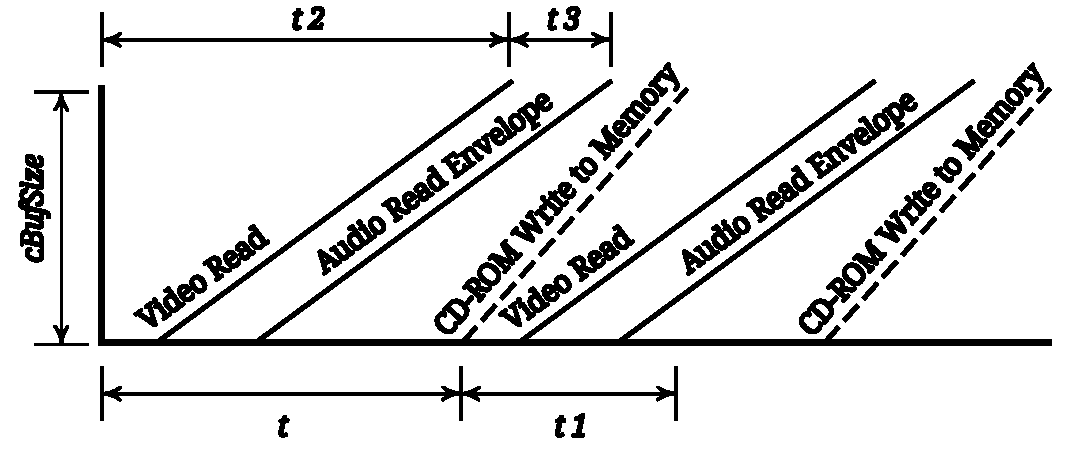
\includegraphics[width=0.6\textwidth]{figures/12/figure_5-a-restored.pdf}
\end{minipage}
\caption{Pointer trajectories vs. time in circular buffer.}
\label{fig:pointer-trajectories-vs-time-in-cbuf}
\end{figure}
\FloatBarrier

Referring to Figure \ref{fig:pointer-trajectories-vs-time-in-cbuf}, we define four times of interest:
\begin{itemize}[nosep, left=0pt .. 36pt]
\item $t$ = zero-based time at which writing of CD-ROM data is initiated;
\item $t1$ = time interval required to fill circular buffer;
\item $t2$ = zero-based expiration time for current video data in circular buffer;
\item $t3$ = lag between audio read envelope and trajectory of video read.
\end{itemize}

The heuristics of the buffer management process are as follows:
\begin{itemize}[nosep, left=0pt .. 36pt]
\item Writing must be initiated late enough that the write pointer does not cross the tail end of the audio read envelope;
\item Writing must be initiated soon enough that there is sufficient backlog of fresh data in the circular buffer at the time the video read pointer is reset.
\end{itemize}

In terms of the above-defined time values, these constraints translate to:
\begin{equation}
\mathrm{t} + \mathrm{t1} > \mathrm{t2} + \mathrm{t3}
\end{equation}
\begin{equation}
\mathrm{t} < \mathrm{t2}
\end{equation}

Solving both inequalities for $t2 - t$ and rearranging, we obtain the concise result:
\begin{equation}
0 < \mathrm{t2} - \mathrm{t} < \mathrm{t1} - \mathrm{t3}
\end{equation}

The most conservative design strategy is to split the difference, i.e.
\begin{equation}
\mathrm{t2} - \mathrm{t} = \frac{\mathrm{t1} - \mathrm{t3}}{2}
\end{equation}

this is the approach which has been taken in the sample player code.

The combination $(t1 - t3)/2$ is referred to as \texttt{deltaTime} in the sample code (see also Table \ref{tab:keyvar}). The value is computed halfway between labels \texttt{CalcDest} and \texttt{.ClearWindow} in \texttt{player.s}. The comparison between $t2 - t$ and \texttt{deltaTime} is made just after label \texttt{CheckCDPlay}, once it is determined that \texttt{playPhase = 0}.

The mechanics of transferring CD-ROM data to the circular buffer are all managed by the GPU interrupt service routine, which is loaded by an initial call to the CD-BIOS routine \texttt{CD\_init}; this call is made as part of the \texttt{LoadGPU} subroutine in module \texttt{utils.s} (see Table \ref{tab:utilities}). Subroutine \texttt{ReadCDData} takes care of all the overhead associated with setting up the BIOS calls to access the CD-ROM, including specification of an ``end-of-buffer'' address. When the write pointer has advanced to this address, the transfer of data is automatically suspended until the next call to \texttt{ReadCDData}; no further intervention by the playback code is required.

\subsection{Frame Rate Control}
The mechanism for frame rate control is fairly simple. The sample record (see Table \ref{tab:samplerec}) contains a field which indicates the scheduled time for the sample. The clock time, maintained by the vertical interval interrupt, is compared with the scheduled time and the system waits until the two times are the same. The code for doing this appears in \texttt{player.s} at label \texttt{KillTime}.

If the display of video falls behind schedule by an amount greater than \texttt{maxDelay}, then the \texttt{catchUp} flag is set and frames are skipped until the next key frame is encountered. When this occurs, the \texttt{catchUp} flag is cleared, the key frame is displayed and normal operation resumes. This code appears six to eight instructions on either side of label \texttt{LookForKey} in \texttt{player.s}.

Under most circumstances, there is ample processing power in the system to play full-screen video at 24 or even 30 frames per second, so the catch-up mode will seldom be activated. However, there may be situations in which developers will also want to use some portion of the GPU processing bandwidth for purposes other than video decompression; in these cases, the catch-up mechanism is essential.

\subsection{Code Walkthrough}
In this section, we give a complete walkthrough of the sample code in \texttt{player.s}, highlighting major points of interest along the way.

Before beginning, we define in Table \ref{tab:registers} the use of several dedicated 68000 registers; this will clarify some of the explanations as we progress. All other registers are available for scratchpad computations.

\begin{table}[h]
\centering
\begin{tabular}{|c|p{12cm}|}
\hline
\rowcolor{black}
\tabheadtxt{Register} & \tabheadtxt{Use} \\
\hline
d4 & Pointer to compressed frame data \\
\hline
d5 & Counter for samples remaining in chunk \\
\hline
d7 & Counter for chunks remaining in circular buffer \\
\hline
a3 & Pointer to current sample record in circular buffer \\
\hline
a4 & Pointer to start of current chunk in circular buffer \\
\hline
a5 & Pointer to current chunk record in chunk table \\
\hline
\end{tabular}
\caption{Dedicated 68000 registers in film player code.}
\label{tab:registers}
\end{table}
\FloatBarrier

Between the start of the code and the label \texttt{WaitGPU}, the system is initialized. Much of the code used here -- especially in subroutines -- is either identical to, or a close derivative of early versions of generic Jaguar sample code distributed by Atari. Note, however, that some aspects of this code are no longer considered to be good examples of general Jaguar programming.

The \texttt{Lister} subroutine has been modified to store certain entries in the object list in memory for subsequent use by the vertical interrupt interrupt service routine.

The \texttt{USE\_CDROM} switch, set at assembly time, allows assembly of code that bypasses all access to CD-ROM; this is useful during development for testing short (three- or four-second) films by downloading them into memory from the hard disk.

After the GPU has finished initialization, the first access to the CD-ROM occurs. Data from the CD-ROM will be read into memory starting at location \texttt{FILM\_BASE}. At label \texttt{.ClearWindow}, we allow the write pointer to advance beyond the end of the sync search window, then call \texttt{FindSync} to locate the start of the film. At label \texttt{CheckFilm}, we verify that the frame header tag (see Table \ref{tab:framehead}) follows the film sync.

At labels \texttt{RelocTable} and \texttt{CopyCT}, the entire chunk table is moved from wherever it happened to land in the buffer to location \texttt{FILM\_BASE}. Next, the \texttt{mediaOffset} variable is computed, since the byte offset for all subsequent accesses to CD-ROM data will be relative to the end of the chunk table. Following this, \texttt{cBufBase} and \texttt{cBufSize} are determined: the size of the chunk table is subtracted from the total available memory and whatever is left is allocated to the circular buffer. The \texttt{cType} field in the frame description atom is tested and the video is switched to CRY if the CRY tag is found.

The value of \texttt{dest} is computed at label \texttt{CalcDest}. In the sample code, the film is centered on the display; developers will obviously want to adapt this for their own purposes. After this, the \texttt{filmChunks} variable is initialized by copying the value from the \texttt{Count} field of the chunk table (see Table 3.10). Next, three key time variables are computed: \texttt{timeIncr}, \texttt{maxDelay} and \texttt{deltaTime}. Finally, register a5 is set to point to the first chunk record (see Table \ref{tab:registers}).

We are now ready to look for the first chunk in the circular buffer. The search begins at \texttt{cBufBase}, with a sync pattern given by \texttt{\$c(a5)}. At label \texttt{.ClearWindow}, we again wait to ensure that the write pointer has advanced beyond the end of the search window before calling \texttt{FindSync}. Upon returning from \texttt{FindSync}, we verify that the sample table header tag (see Table \ref{tab:sampletab}) follows the chunk sync.

At label \texttt{.ChunkOK}, register a4 is set to point at the start of the chunk and a3 to point at the sample table for the chunk. A call to \texttt{SetNextGroup} is made to determine which chunk will be the target of the next access to CD-ROM.

Two final steps are required before we are ready to play the film. At label \texttt{WaitToFill}, we allow the write pointer to get far enough ahead that the read pointer will not catch up to it. At label \texttt{WaitForTick}, we restart the vertical interval time clock at zero, since all time references in the film file are zero-based.

Label \texttt{ChunkLoop} is the top of the outer program loop. Register d5 is loaded from the \texttt{Count} field of the sample table (see Table \ref{tab:sampletab}). The \texttt{AtomSize} field of the sample table is added to the base address of the sample table in a3 to determine the address of the first data sample in the chunk; this is transferred to d4. Next, a3 is adjusted to point to the current sample record.

Label \texttt{SampleLoop} is the top of the inner program loop. The call to \texttt{Snapshot} generates a time history in ROM emulator address space which is very useful for doing post-mortems during development; it should be commented out or deleted in production versions of the code. The \texttt{Time} field of the sample record is tested to determine whether the sample is audio or video. If it is audio, the arguments specified in Section 5.6 are passed to the DSP and a branch is taken to the end of the sample loop; otherwise, the program falls through to process video.

At labels \texttt{DoVideo} and \texttt{KillTime}, the \texttt{Time} field of the sample record is read and compared with the current time variable. If we are ahead of schedule, we wait until time has advanced to the scheduled value; otherwise, we check to see how far behind schedule we have fallen. If the slip exceeds the time specified by \texttt{maxDelay}, we begin the catch-up process described in Section 5.9; otherwise, we proceed to display the frame. The stack setup for the call to \texttt{CheckKeyFrame} is specified in Table \ref{tab:checkKeyFrame}.

The call to \texttt{ForceDelay} at label \texttt{DisplayFrame} can be conditionally assembled to simulate the catch-up process during development; there is no other use for \texttt{ForceDelay}. Next the stack is set up for the call to \texttt{PreDecompress} (see Table \ref{tab:predecompress}). Following the return, an error check is performed on the return value. At label \texttt{StartDecomp}, the stack is prepared for the call to \texttt{Decompress} (see Table \ref{tab:decompress}); error checking is likewise performed upon return.

All of the code which manages the dynamics of writing to the circular buffer (excluding the initial write) appears between labels \texttt{CheckCDPlay} and \texttt{NextSample}. The \texttt{playPhase} variable, described in Table 5.2, is the key to controlling this mechanism:

\begin{itemize}[nosep, left=0pt .. 36pt]
\item When \texttt{playPhase} is 0, the CD-ROM is not playing and the only task is to check the difference between the expiration time and the clock time and compare this difference with \texttt{deltaTime}. Note that the expiration time is recovered from the \texttt{Time} field of the chunk record which is addressed by \texttt{pNextChunk}. If it is time to start filling the buffer, the CD-ROM is given a seek address determined by the \texttt{Start} field of the chunk record pointed to by \texttt{pNextChunk}, playing is initiated with a write destination of \texttt{cBufBase}, and \texttt{playPhase} is set to 1; otherwise, a branch is taken to \texttt{NextSample}.

\item When \texttt{playPhase} is 1, the CD-ROM is playing, and the only task is to locate the start of the next group of chunks in the circular buffer. Before calling \texttt{FindSync}, a test is performed to see if the write pointer has progressed beyond the end of the sync search window. If the test fails, the program does not wait, but branches to \texttt{NextSample}; this is to avoid needless delay in the middle of a loop that must execute in real time. If the test passes, the following actions are taken:
  \begin{itemize}[nosep]
  \item The sync search is begun at \texttt{cBufBase}, with a sync pattern specified by the \texttt{SyncPattern} field of the chunk record addressed by \texttt{pNextChunk},
  \item Error checking is performed;
  \item The \texttt{nextBufAddr} variable is set at the sync location in the circular buffer and \texttt{SetNextGroup} is called to determine which chunk will be the target of the subsequent access to CD-ROM;
  \item \texttt{playPhase} is set to 2.
  \end{itemize}
\end{itemize}

Once \texttt{playPhase} has reached 2, there is nothing further to be done until the count (d7) of chunks currently in the circular buffer is exhausted. This situation is handled following label \texttt{ResetBuffer} (see below).

At label \texttt{NextSample}, the \texttt{Size} field of the current sample record is added to the address (d4) of the current sample to obtain the address of the next sample, and the pointer (a3) to the sample record is advanced to the next record. The counter (d5) for the number of samples in the current chunk is decremented, and if not exhausted, a backward branch is taken to \texttt{SampleLoop}.

If the sample count (d5) is exhausted, the counter (d7) for the number of chunks remaining in the buffer is decremented. If there are no chunks left, a branch is taken to \texttt{ResetBuffer}; otherwise, the \texttt{Size} field of the current chunk record is added to the address (a4) of the current chunk to obtain the address of the next chunk in the buffer, and register a3 is set to point at the sample table for the next chunk. At this point, a test is made for an empty chunk (no video or audio scheduled) and a backward branch is taken to either \texttt{ChunkLoop} (not empty) or \texttt{NextChunk} (empty).

At label \texttt{ResetBuffer}, d7 is reloaded from the \texttt{buffChunks} variable, which is set either in \texttt{SetNextGroup} or a few instructions below. If the value loaded is zero, the film is finished and we branch to \texttt{Done}.

For a nonzero value, a5 is advanced to the next chunk record, a4 is loaded from \texttt{nextBufAddr}, a3 is set up to point to the sample table for the first sample in the new chunk, and \texttt{playPhase} is reset to zero. Next, the \texttt{filmChunks} variable (maintained by \texttt{SetNextGroup}) is tested to see if there are any chunks beyond those about to be processed that must be loaded from the CD-ROM. If so, a backward branch is taken to \texttt{ChunkLoop}.

If not, \texttt{playPhase} is set to 3 and \texttt{buffChunks} is set to zero. The first action inhibits any further access to the CD-ROM; the second causes the program to terminate when the current group of chunks has been exhausted. A backward branch is then taken to \texttt{ChunkLoop} to finish playing the film.

\subsection{Error Trapping}
There are several error conditions related to CD-ROM data integrity which are checked by the 68000 and trapped via an illegal instruction. When the trap is taken, register d0 will contain an error code, according to the condition which caused the trap. Table \ref{tab:errorcodes} summarizes the traps and condition codes.

\begin{table}[h]
\centering
\begin{tabular}{|c|p{12cm}|}
\hline
\rowcolor{black}
\tabheadtxt{Code} & \tabheadtxt{Condition} \\
\hline
\$00000000 & No error; playback completed normally \\
\hline
\$11111111 & Sync pattern not found within search window \\
\hline
\$22222222 & 'FILM' tag not found at start of film header \\
\hline
\$33333333 & 'STAB' tag not found at start of sample table \\
\hline
\$44444444 & Data error detected by PreDecompress \\
\hline
\$55555555 & Data error detected by Decompress \\
\hline
\end{tabular}
\caption{Error codes and conditions.}
\label{tab:errorcodes}
\end{table}
\FloatBarrier

These traps are useful for development and experimentation. They should never occur during playback of a finished Jaguar film.

\section{Sample Jaguar Films}
Three sample Jaguar films are provided on CD-ROM for demonstration purposes; any of the three films can be played using the sample code without modification. The film material has been approved for distribution and can be freely used for demonstration or evaluation.

Table \ref{tab:samplefilms} summarizes the characteristics of the three sample films:

\begin{table}[h]
\centering
\begin{tabular}{|l|l|l|l|}
\hline
\rowcolor{black}
 & \tabheadtxt{Excerpt from "Jaws"} & \tabheadtxt{"Escape" sequence} & \tabheadtxt{Excerpt from "Back}\\
\rowcolor{black}
 & & \tabheadtxt{ from Star Wars} & \tabheadtxt{ To the Future 3"}\\
\hline
Resolution & 288 x 136 & 288 x 216 & 288 x 216\\
\hline
Pixel depth & 16 bits & 16 bits & 16 bits\\
\hline
Color format & Cinepak RGB & Cinepak RGB & Cinepak RGB\\
\hline
Frame rate & 24 fps & 24 fps & 24 fps\\
\hline
Compressed video rate & 220 kB/sec & 260 kB/sec & 280 kB/sec\\
\hline
Audio sample rate & 22251.5 Hz & 22251.6 Hz & 22249 Hz\\
\hline
Chunk duration & 1.0 sec & 0.5 sec & 0.5 sec\\
\hline
Film duration & 2:33 min & 1:09 min & 1:08 min\\
\hline
\end{tabular}
\caption{Sample Jaguar films.}
\label{tab:samplefilms}
\end{table}
\FloatBarrier

All CD-ROMs are single-session with the film data recorded on track zero. This is the format expected by the sample player code.

\section{Notice}
Cinepak is a registered trademark of Radius, Inc. Jaguar is a registered trademark of Atari Corporation. QuickTime, Macintosh and MPW are registered trademarks of Apple Computer, Inc. Think C is a registered trademark of Symantec Corporation. COSA and After Effects are registered trademarks of The Company of Science and Art.

\section{Jaguar Cinepak Utility For Macintosh}

The \titformat{Jaguar Cinepak Utility} program runs on the Apple Macintosh under System 6.1 or later
(older versions of System/Finder may work, but have not been tested). The QuickTime extensions must
also be loaded. When you run the program, you'll see a screen that looks like this:

\begin{figure}[h]
\centering
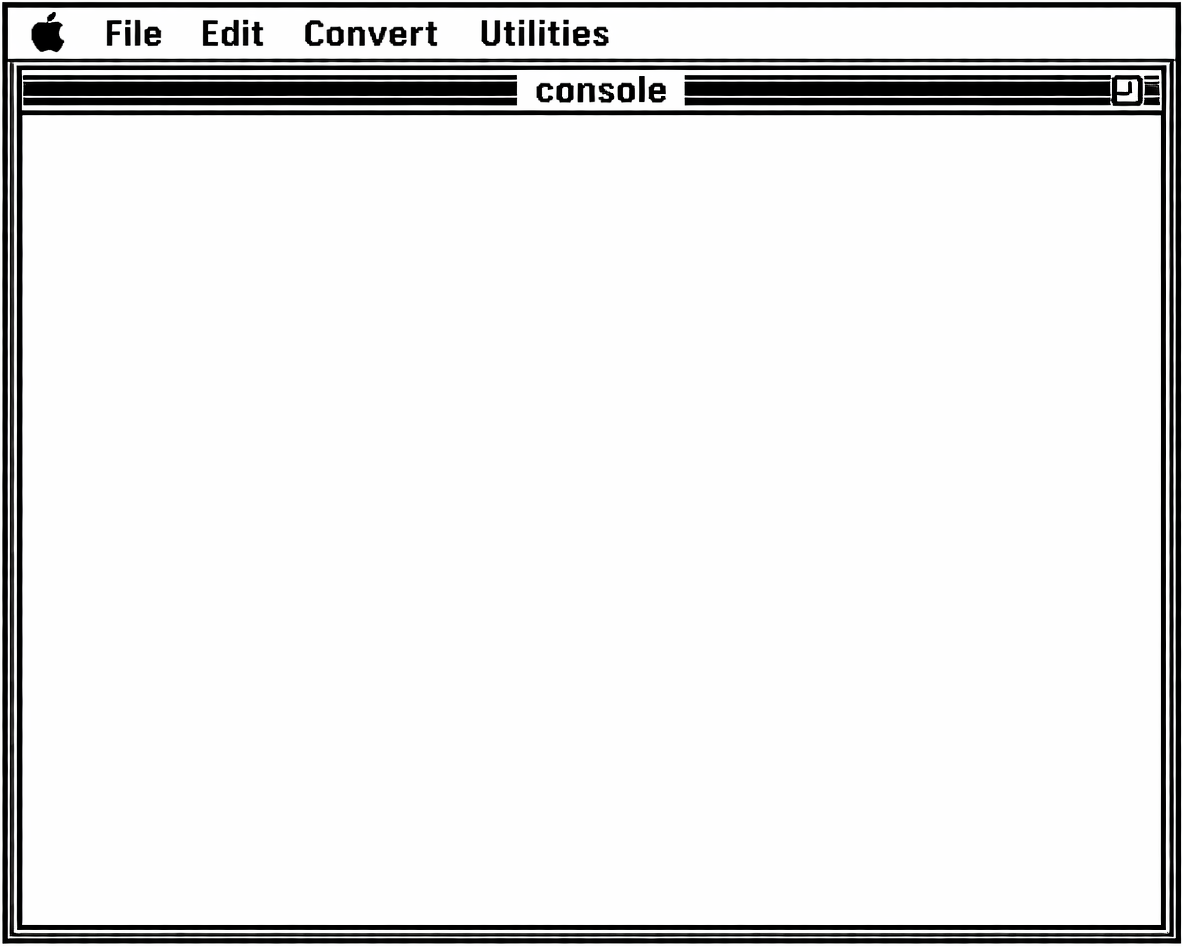
\includegraphics[width=0.6\textwidth]{figures/12/figure_8-a-restored.png}
\caption{Jaguar Cinepak Utilities Screen}
\label{fig:jaguar-cinepak-utilities-screen}
\end{figure}
\FloatBarrier

We'll assume that you know how to run programs and generally use the Macintosh computer. If this
isn't true, please look through your Macintosh user's manual before attempting to run the
\titformat{Jaguar Cinepak Utility}.

The program displays a console window where messages from the various conversion functions will
appear, as well as a menu bar at the top. The menus and the items they contain are described below.

\subsection{File Menu}

The \textit{File} menu has just a single choice that allows you to quit the program.

\subsection{Edit Menu}

The Edit menu has the standard list of choices for Cut, Copy, Clear, and Paste. However, these
options are not yet functional in this version of the utility. In future versions, they will allow
you to edit the text shown in the console window.

\subsection{Convert Menu}

There are six conversion options available in the \textit{Convert} menu. The first four are:
\textit{Movie To Film}, \textit{RGB To Cry}, \textit{Smooth To Chunky}, and \textit{Film To AIFF}.
These described in additional detail below.

The last two choices are \textit{Convert A QuickTime Movie} and \textit{Convert QuickTime Movie
Batch}. These options allow you to combine the individual conversion steps represented by the top
four menu choices. This is discussed in further detail below.

\subsection{Utilities Menu}

There is also a \textit{Utilities} menu with options for displaying information about Jaguar Cinepak
Film files and QuickTime movie files. These are discussed further detail below.

\subsection{Movie To Film}

The \textit{Movie To Film} function allows you to convert a standard QuickTime Cinepak movie to the
smooth Jaguar film format. Selecting this menu item leads to a dialog box that allows you to select
the input file and the output file and conversion options as shown below:

\begin{figure}[h]
\centering
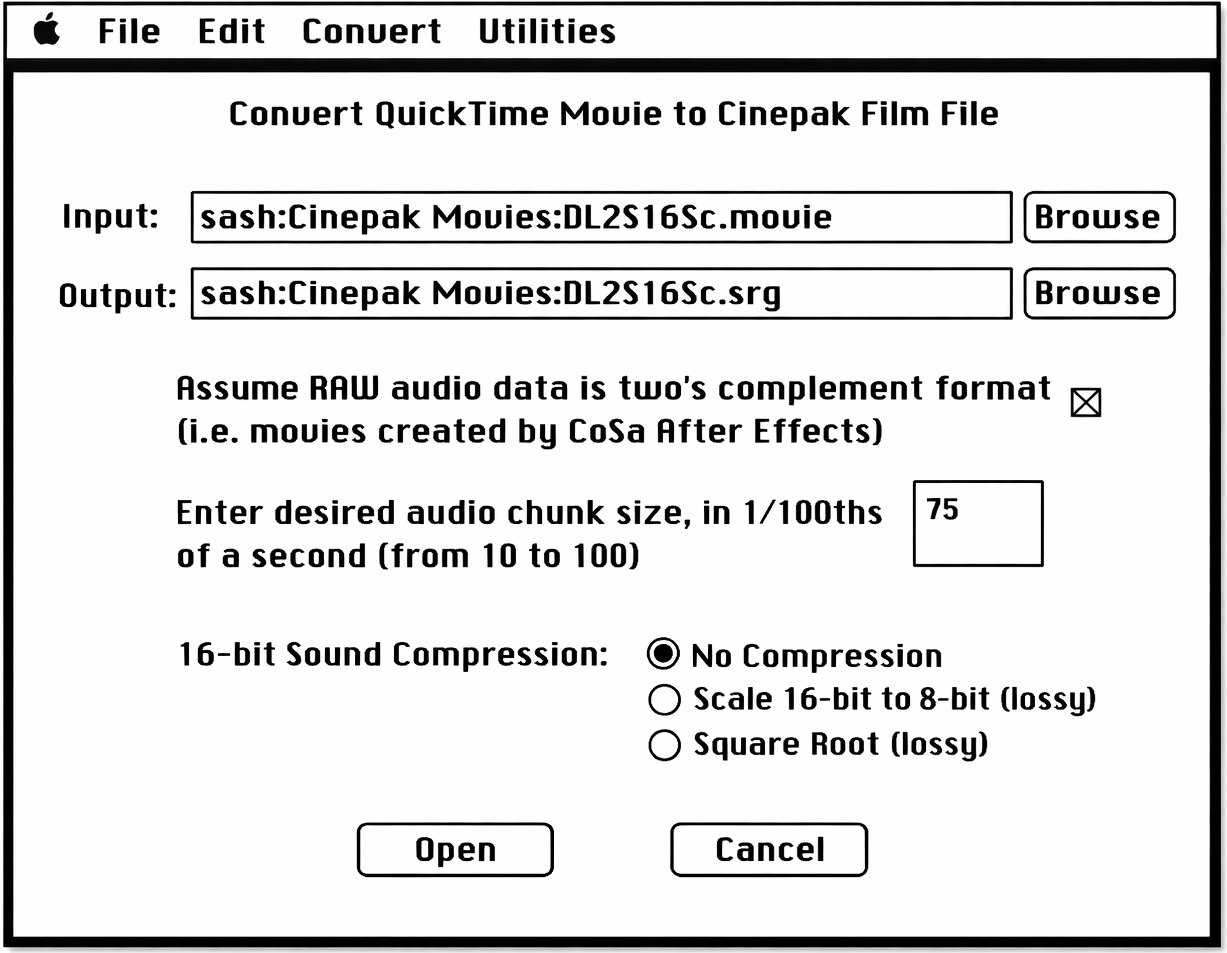
\includegraphics[width=0.7\textwidth]{figures/12/figure_8-b-restored.png}
\caption{\textit{Movie To Film} dialog}
\label{fig:movie-to-film-dialog}
\end{figure}
\FloatBarrier

The input file must be an existing QuickTime Cinepak movie. You can type in the name of the file
yourself, or you can click on the \textbf{Browse} button at the end of the \textbf{Input} field and
the standard Macintosh file selector will appear and allow you to select the desired filename. In
the event that the \textbf{Output} field is blank when you \textbf{Browse} for the input field, the
input filename you select will be used to guess at the desired output filename. You may either use
the guess directly or edit it as required.

The output file name may be specified by typing in a name or by selecting the \textbf{Browse} button
and using the standard Macintosh file selector that appears. Any existing file with the same name as
the output file will be overwritten. If you use the file selector to enter the output filename, you
will be given a warning, but not if you simply type it in. \textit{Note: Using a filename extension
of ``\texttt{.SRG}'' is recommended.}

The \textit{Assume RAW Audio Data\ldots} checkbox allows you to inhibit the conversion of ``Raw''
audio tracks in the source QuickTime movie to the ``Two's Complement'' format needed for proper
playback on the Jaguar.\footnote{QuickTime movies typically specify either a ``RAW'' audio track or
a ``Two's Complement'' audio track. The ``Raw'' type is normally the binary-offset format that is
the default audio format used by the Macintosh. However, ``Raw'' also means the actual data format
is not precisely defined, and some ``Raw'' audio tracks may not require conversion. This is the case
with movies created by \textit{Adobe (CoSA) After Effects}, for example. Selecting the \textit{Assume
RAW Audio Data\ldots} checkbox will inhibit the conversion of ``Raw'' audio tracks.

QuickTime movies that specify a ``Two's Complement'' audio track will normally not be converted
regardless of the checkbox setting. However, if you hold down the Shift+Command keys on the
keyboard when selecting the menu choices \textit{Movie To Film}, \textit{Convert A QuickTime Movie},
or \textit{Convert QuickTime Batch}, these tracks will be converted if the checkbox is not selected.
(Remember, the checkbox says ``the audio is already Two's Complement, leave it alone.'')}

Audio data from the source movie is placed into the destination file in chunks interleaved with the
video data. The length of each audio chunk is specified by the \textit{Enter Audio Chunk Size\ldots}
edit box. This value is specified as $n/100$ths of a second, and should ordinarily be about $3/4$
the size of the chunk size you will later specify in the \textit{Smooth To Chunky} conversion
process. The default size is $75/100$ths of a second. Note that the actual amount of data placed
into the audio chunk depends on the format of the audio data. If you use 16-bit stereo audio it
will take 4 bytes per sample, versus 1 byte per sample for 8-bit mono.

Assuming an audio chunk size of $75/100$ths of second, and video running at 24 frames per second,
the audio will be placed into the destination file in the following way: the first audio chunk will
be placed in the destination file immediately after the first frame of video. The second audio chunk
will be inserted after video frame \#10. The remaining audio chunks will be inserted every 18 video
frames. This forward temporal bias in the audio stream means that the audio will play interrupted,
as we will always have a little more audio remaining in the buffer than we have video, even in cases
where the video playback starts to lag behind real time.

You may specify audio chunk sizes from $10/100$ths to 1 second. If you later specify chunk sizes
less than 1.0 seconds long in \textit{Smooth To Chunky}, you should reduce the audio chunk size
accordingly. However, please note that changing the audio chunk size to less than $3/4$ of the
chunk size later specified in \textit{Smooth To Chunky} may affect the audio playback of the movie.
If you have problems, try increasing the audio chunk size.

If the source QuickTime movie has a 16-bit audio track, then you have the option of compressing the
audio data. There are two ways to do this. The first method is to simply scale the 16-bit samples
to 8-bit. The second method uses a special square root compression algorithm. Each 16-bit audio
sample is converted to an 8-bit encoded value as follows:

\begin{center}
\texttt{8-bit encoded value = sqr(original sample value / 2)}
\end{center}

The 8-bit encoded values are then placed into the destination film file. During playback, these
encoded sample values are expanded back to 16-bit. This compression method is still lossy (i.e.\ the
output is not quite the same as the input), but the results are usually more pleasing to the ear
than simply scaling 16-bit values to 8-bit.

The actual \textit{Movie To Film} conversion process is also accessed through the \textit{Convert A
QuickTime Movie} and \textit{Convert QuickTime Batch} options.

\subsection{RGB To CRY}

The \textit{RGB To CRY} function expands Cinepak-compressed RGB video data in a smooth format Jaguar
Cinepak film to either CRY or RGB uncompressed. The movie's smooth film structure is not changed.

\begin{figure}[h]
\centering
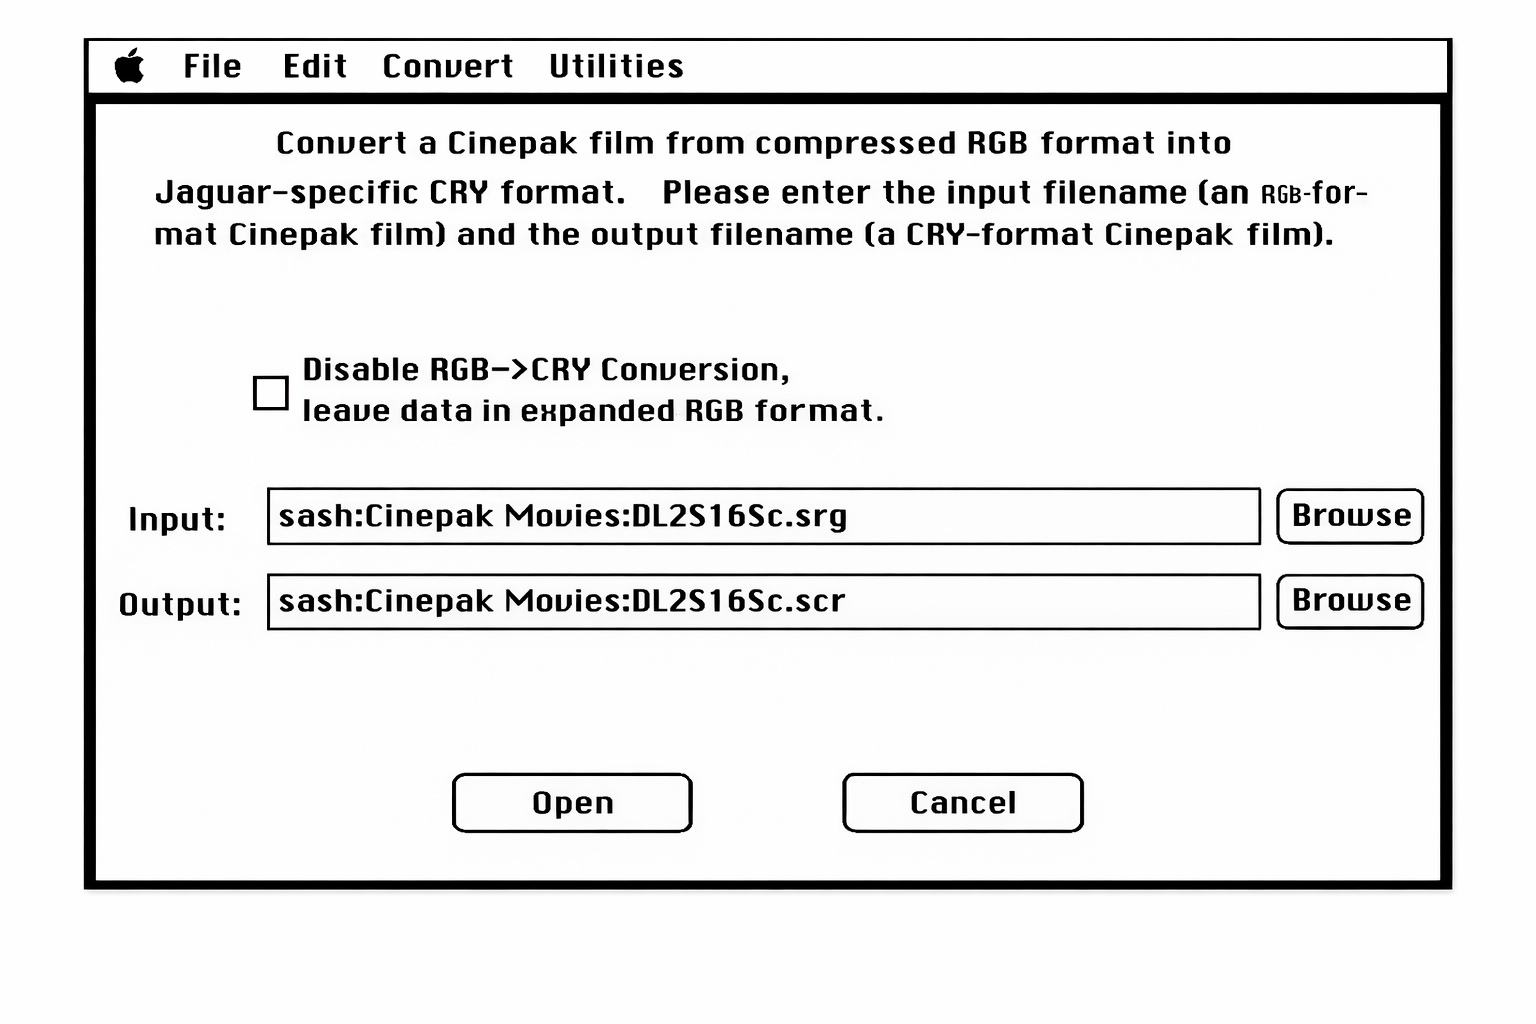
\includegraphics[width=0.7\textwidth]{figures/12/figure_8-c-restored.png}
\caption{\textit{RGB to CRY} dialog}
\label{fig:rgb-to-cry-dialog}
\end{figure}
\FloatBarrier

The \textit{RGB To CRY} function converts a smooth-format Jaguar film from the Cinepak
compressed-RGB color format to either the Atari Jaguar CRY format, without altering the smooth film
structure. Selecting this menu item will lead to a dialog box where you can select the input file,
output file, and conversion options.

The input file must be an existing Jaguar Cinepak film in compressed-RGB format previously converted
with \textit{Movie To Film}. You can type in the name of the file yourself, or you can click on the
\textbf{Browse} button at the end of the \textbf{Input} field and the standard Macintosh file
selector will appear and allow you to select the desired filename. In the event that the
\textbf{Output} field is blank when you \textbf{Browse} for the input field, the input filename you
select will be used to guess at the desired output filename. You may either use the guess directly
or edit it as required.

The output file name may be specified by typing in a name or by selecting the \textbf{Browse} button
and using the standard Macintosh file selector that appears. Any existing file with the same name as
the output file will be overwritten. If you use the file selector to enter the output filename, you
will be given a warning, but not if you simply type it in. \textit{Note: Using a filename extension
of ``\texttt{.SRG}'' is recommended for movies with RGB video, or ``\texttt{.SCR}'' for movies with
CRY video.}

The \textit{RGB To CRY} function first decompresses the proprietary Cinepak RGB color data to a
non-compressed RGB format. Checking the \textit{Disable RGB->CRY Conversion\ldots} checkbox
disables the final conversion of this data to CRY mode.

Note that the decompression operation performed by \textit{RGB To CRY} increases the amount of data
needed to represent each frame of video, so various entries in the header and sample table are also
adjusted to reflect the change. The increase in size of the resulting film is typically about 10\%,
so there is minimal penalty in either storage or CD-ROM access requirements.

Cinepak films using non-compressed RGB or CRY video will consume about 10--15\% less GPU processing
bandwidth on playback than the same film using compressed-RGB video. The reason is that the
processing step which converts from compressed to expanded RGB is bypassed (having already been done
off-line). For certain highly complex movies where the frame rate may fall slightly short of 24 fps,
developers may wish to take advantage of this time savings in order to squeeze maximum performance
out of the system.

The actual \textit{RGB To CRY} conversion process is also accessed through the \textit{Convert A
QuickTime Movie} and \textit{Convert QuickTime Movie Batch} options.

\subsection{Smooth To Chunky}

The \textit{Smooth To Chunky} menu item converts a Jaguar film from the smooth file format to the
chunky format. Selecting this menu item will lead to a dialog box where you can select the input
file, output file, and conversion options.

\begin{figure}[h]
\centering
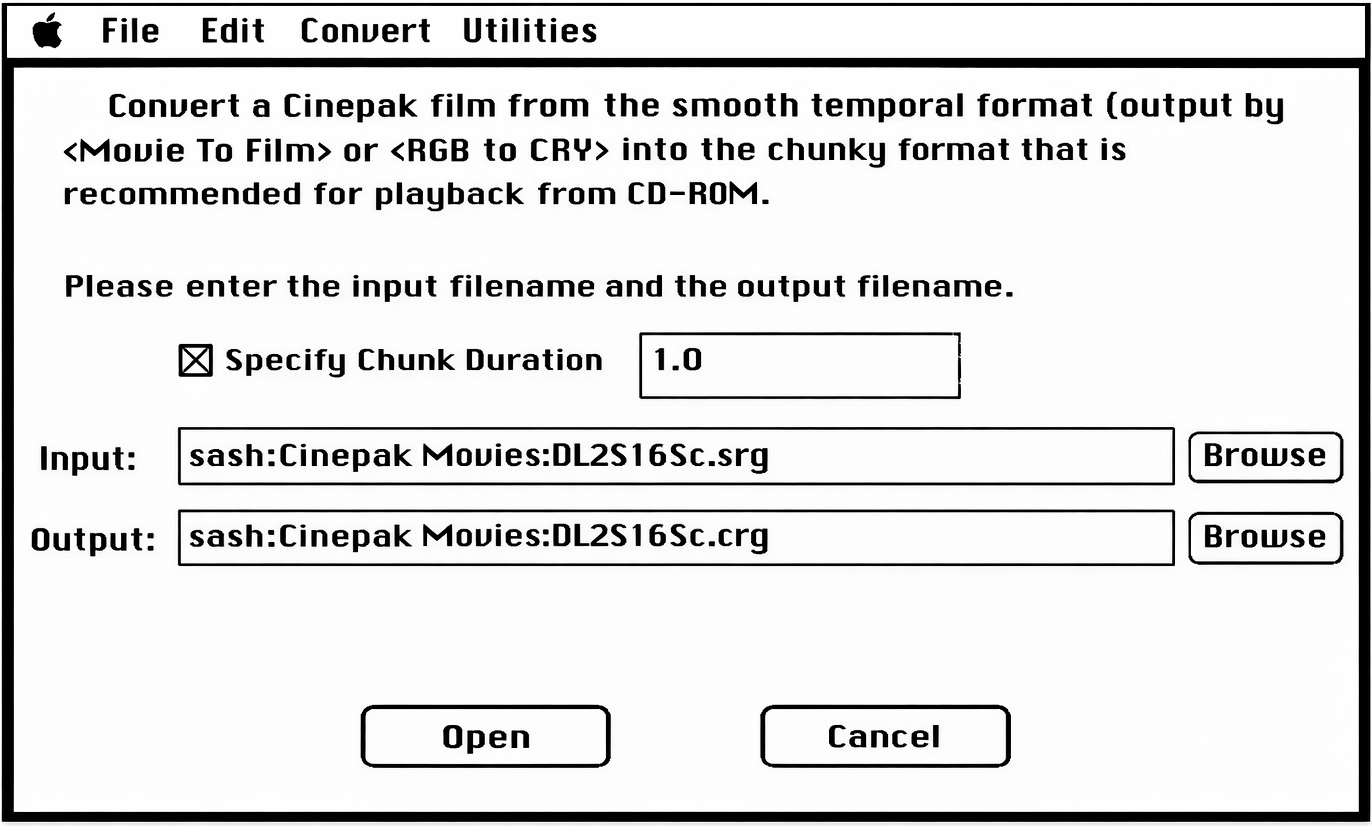
\includegraphics[width=0.7\textwidth]{figures/12/figure_8-d-restored.png}
\caption{\textit{Smooth To Chunky} dialog}
\label{fig:smooth-to-chunky-dialog}
\end{figure}
\FloatBarrier

The input file must be an existing smooth-format Jaguar Cinepak film previously created by either
\textit{Movie To Film} or \textit{RGB To CRY}. You can type in the name of the file yourself, or
you can click on the \textbf{Browse} button at the end of the \textbf{Input} field and the standard
Macintosh file selector will appear and allow you to select the desired filename. In the event that
the \textbf{Output} field is blank when you \textbf{Browse} for the input field, the input filename
you select will be used to guess at the desired output filename. You may either use the guess
directly or edit it as required.

The output file name may be specified by typing in a name or by selecting the \textbf{Browse} button
and using the standard Macintosh file selector that appears. Any existing file with the same name as
the output file will be overwritten. If you use the file selector to enter the output filename, you
will be given a warning, but not if you simply type it in. \textit{Note: Using a filename extension
of ``\texttt{.CRG}'' is recommended for movies with RGB video, or ``\texttt{.CCR}'' for movies with
CRY video.}

Checking the \textit{Specify Chunk Duration} checkbox will cause an edit box to appear where you can
specify the chunk duration, in seconds, of each chunk of data that will be placed into the
destination file. If this option is not invoked, a default value of 0.25 seconds is used.

The \textit{Smooth To Chunky} function takes a smooth-format Jaguar Cinepak film and converts it
into a chunky-format Jaguar Cinepak film. This essentially takes audio chunks and frames of video
from the smooth file and places them into chunks of a particular playback duration.

See sections 3 to 3.2 for further information on the smooth and chunky Cinepak film formats.

A chunk never begins with audio; an audio block which happens to fall on a chunk boundary is always
incorporated as the final data element in the earlier of the two chunks.

The global chunk table is inserted near the beginning of the file, following the frame description
atom. Synchronization blocks and local (i.e.\ intra-chunk) sample tables are inserted at the
beginning of the film data for each chunk. This is so that the data for each individual chunk may
be reliably located when reading from CD-ROM.

Developers are free to experiment with the chunk duration. On the low end, the value is limited by
the increase in the length of the chunk table, which must be stored in its entirety in DRAM. On the
high end, the duration is limited by increasingly inefficient use of DRAM buffer space. Incomplete
chunks at the end of the circular buffer constitute wasted storage; the fraction of wasted buffer
space will increase with progressively larger chunk durations.

The actual \textit{Smooth To Chunky} conversion process is also accessed through the \textit{Convert
A QuickTime Movie} and \textit{Convert QuickTime Movie Batch} options.

\subsection{Film To AIFF}

\begin{technote}
\raisebox{-1.5cm}{
\includegraphics[width=1.8cm]{aux/warning_triangle.pdf}}
\hspace{0.5em}
\parbox[t]{0.75\textwidth}{\emph{\textbf{Warning!}} The \emph{FilmToAIFF} option was designed in
response to certain CD Mastering software packages which could not accept a raw binary file and use
it to create a CD track. Note that the files written by \emph{FilmToAIFF} do not follow the standard
Jaguar CD track format specification. Using \emph{FilmToAIFF} is no longer recommended. Use the
\textbf{Jaguar CD Track Creator} program instead. See the information in the \textbf{Jaguar CD
Mastering} section of the \textbf{Jaguar CD-ROM} chapter, as well as section 4.1.1 of this chapter
for additional information.}
\end{technote}

The \textit{Film To AIFF} menu item converts a Jaguar film file to an AIFF file, suitable as input
to CD-ROM recording software which accepts audio files in this format. Selecting this menu item will
lead to a dialog box where you can select the input file, output file, and conversion options.

% PLACEHOLDER: Figure 8-E — Film To AIFF dialog
\begin{figure}[h]
\centering
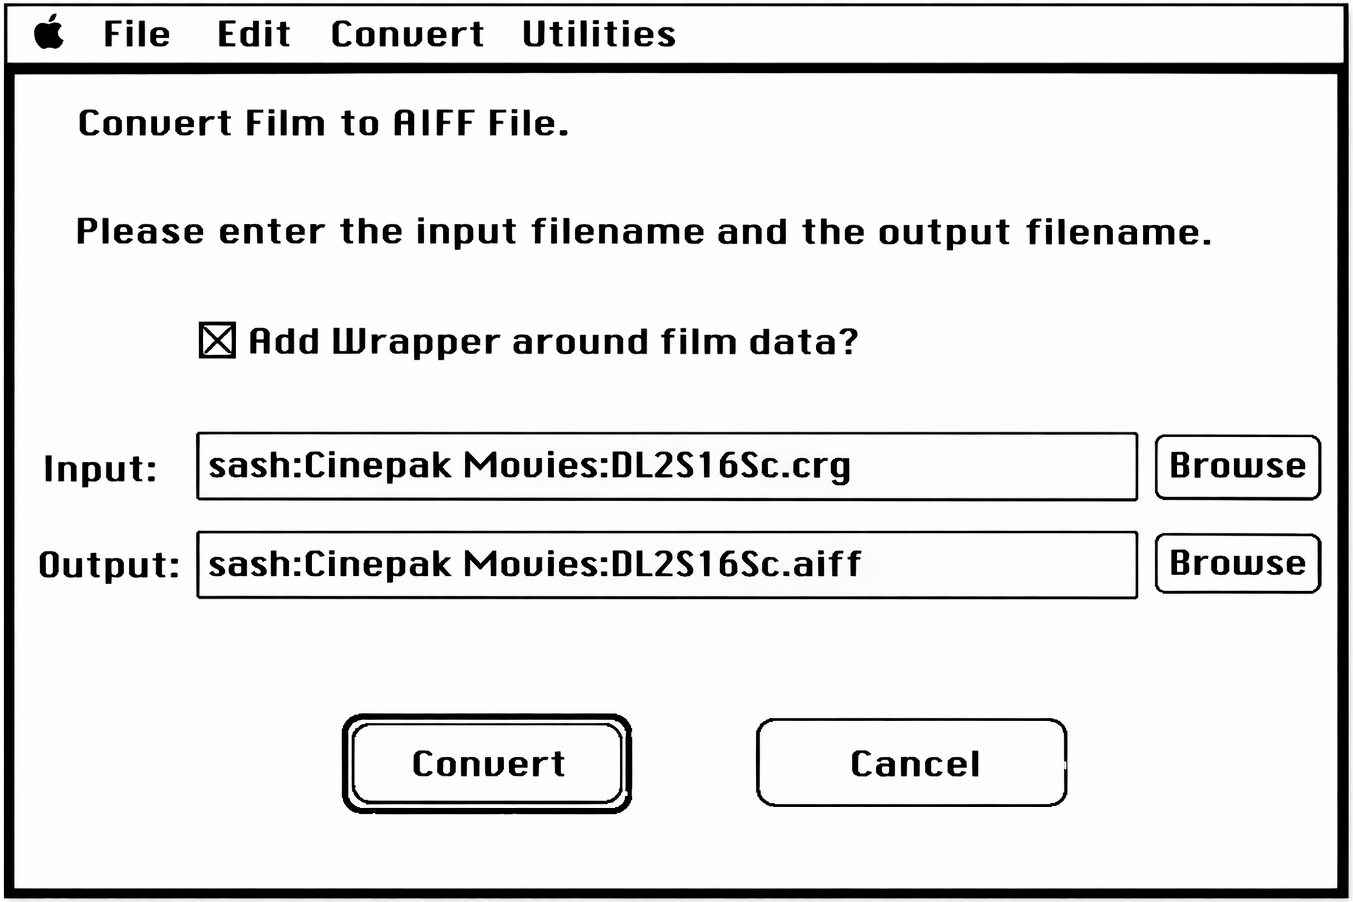
\includegraphics[width=0.7\textwidth]{figures/12/figure_8-e-restored.png}
\caption{\textit{Film To AIFF} dialog}
\label{fig:film-to-aiff-dialog}
\end{figure}
\FloatBarrier

The input file must be an existing Jaguar Cinepak film in either smooth or chunky format created by
\textit{Movie To Film}, \textit{RGB To CRY}, or \textit{Smooth To Chunky}. You can type in the name
of the file yourself, or you can click on the \textbf{Browse} button at the end of the
\textbf{Input} field and the standard Macintosh file selector will appear and allow you to select
the desired filename. In the event that the \textbf{Output} field is blank when you \textbf{Browse}
for the input field, the input filename you select will be used to guess at the desired output
filename. You may either use the guess directly or edit it as required.

The output file name may be specified by typing in a name or by selecting the \textbf{Browse} button
and using the standard Macintosh file selector that appears. Any existing file with the same name as
the output file will be overwritten. If you use the file selector to enter the output filename, you
will be given a warning, but not if you simply type it in. \textit{Note: Using a filename extension
of ``\texttt{.AIFF}'' is recommended.}

There is also a checkbox for an option that is used to cause the film data to be ``wrapped'' by the
header/sync and tailer data structures defined in Table 4.1 before the AIFF file header is added.

This tool is included primarily as a convenience to those developers using CD-ROM mastering software
which cannot do this conversion or which do not accept raw data files as input.

Developers who choose to use or adapt \textit{Film To AIFF} should be aware of three work-arounds
in the code which have been introduced to compensate for bugs in the driver software that was used
in creating the sample CD-ROM:

\begin{itemize}
\item The header and tailer sizes are increased by two bytes each to preserve long alignment of the
film data on the recorded medium (see references to \texttt{HACK\_SIZE} in the definitions of
\texttt{HEAD\_SIZE} and \texttt{TAIL\_SIZE});

\item \texttt{SYNC\_SIZE} is omitted from the computation of \texttt{fileSize};

\item The \texttt{numSampleFrames} field of \texttt{commonChunk} does not correctly account for the
number of channels (=2) and the number of bytes per sample (=2).
\end{itemize}

The latter two work-arounds are needed to prevent spurious failure of the recording process and the
attendant destruction of a CD-ROM.

The actual \textit{Film To AIFF} conversion process is also accessed through the \textit{Convert A
QuickTime Movie} and \textit{Convert QuickTime Movie Batch} options.

\subsection{Convert A QuickTime Movie}

The \textit{Convert A QuickTime Movie} menu item brings up a dialog that combines the functionality of the
separate \textit{Movie To Film}, \textit{RGB To CRY}, \textit{Smooth To Chunky}, and \textit{Film To AIFF} functions into one
place. Please see the documentation for those functions before using \textit{Convert A QuickTime Movie}.

The options in the \textit{Convert A QuickTime Movie} dialog correspond to the options in the separate
\textit{Movie To Film}, \textit{RGB To CRY}, \textit{Smooth To Chunky}, and \textit{Film To AIFF} dialogs with just a few
exceptions, as detailed below.

First, the options currently selected affect the output filename that is automatically created when you
\textit{Browse} the input filename. For example, if you have \textit{RGB Compressed} and \textit{Smooth Film} selected, the
output name will have an extension of ``\texttt{.SRG}''. But if you have \textit{CRY Non-Compressed} and \textit{Chunky
Film} selected, the output name will have an extension of ``\texttt{.CCR}'' instead.

% ---------------------------------------------------------------
%  Figure 8-F  —  Convert A QuickTime Movie dialog
% ---------------------------------------------------------------
\begin{figure}[h]
\centering
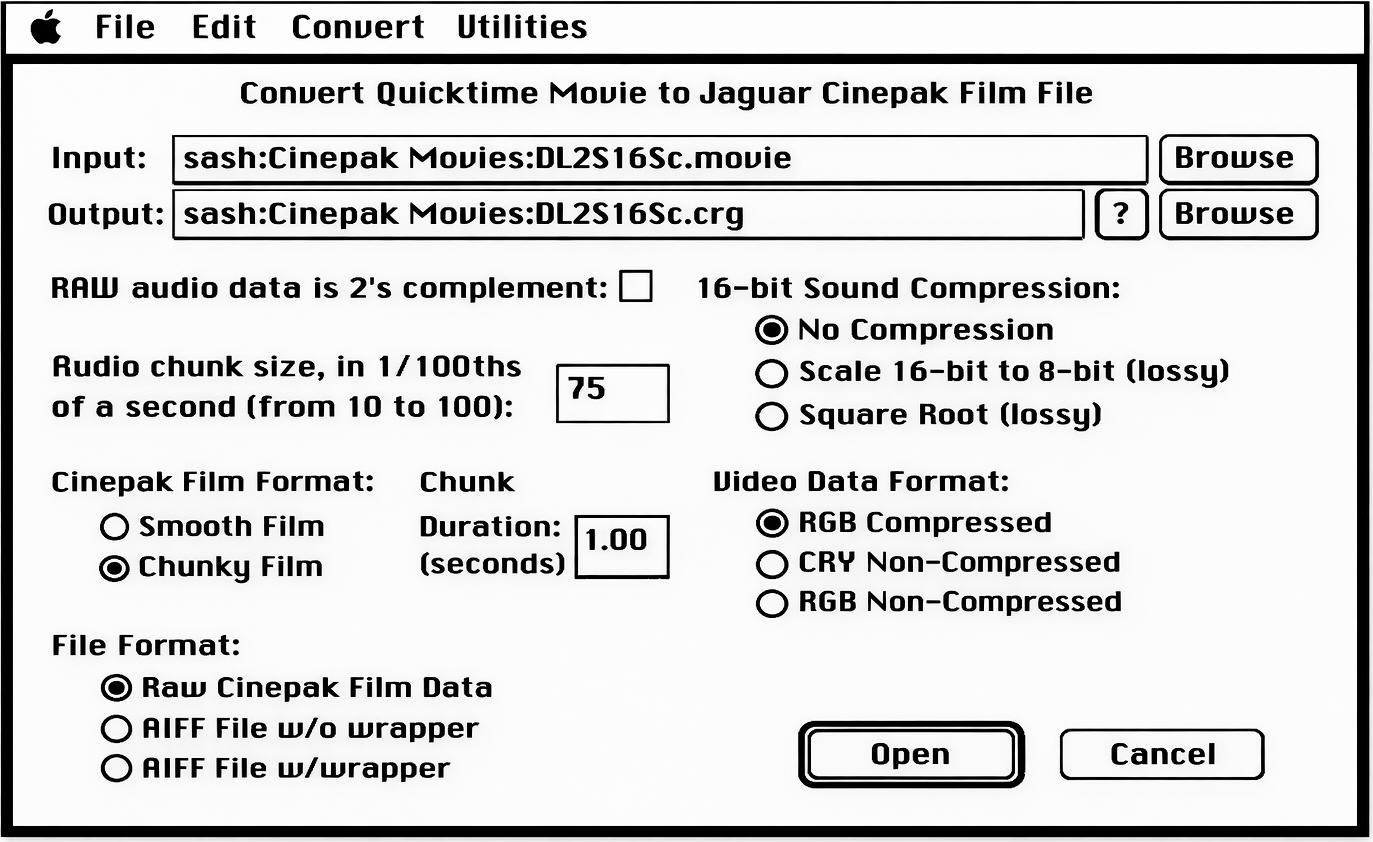
\includegraphics[width=0.7\textwidth]{figures/12/figure_8-f-restored.png}
\caption{\textit{Convert A QuickTime Movie} dialog}
\label{fig:convert-quicktime-movie-dialog}
\end{figure}
\FloatBarrier

In the event you want to change the options after having selected the input filename, you can force the
dialog to recreate the output filename to match the new options by clicking on the ``?'' button next to
the output filename field's Browse button.

Just because the choices are all in one dialog does not change the fact that there are still up to four
separate conversion steps involved. When you exit the dialog, \textit{Convert A QuickTime Movie} will call
the \textit{Movie To Film} conversion as well as whichever of the three other conversion steps are appropriate
for the options you have selected.

Any intermediate files required between the source and final destination will be created and deleted as
needed. You will typically need to have approximately 2.2 times as much free disk space available as
the size of your source movie. Please note that the amount of free disk space is \textbf{\textit{not checked}} prior to
the beginning of the conversion process.

Holding down the SHIFT+COMMAND keys when selecting the \textit{Convert A QuickTime Movie} menu item
will cause the \textit{Raw Audio Data is Two's Complement} checkbox setting to affect QuickTime movies
with the ``twos'' audio format as well as movies with the ``raw'' audio format.

\subsection{Convert QuickTime Movie Batch}

The \textit{Convert QuickTime Movie Batch} menu item brings up a file selector which allows you to select the
filename of a text file containing a list of QuickTime movie files to be converted. This file may be
arbitrarily long and can therefore allow you to process dozens or even hundreds of QuickTime movies
at once.

Each line in the batch file must specify a list of desired options and the source filename. You may also
specify the destination filename, but if none is specified, one will be created based on the conversion
options selected. The available command line options are:

\begin{table}[h]
\centering
\begin{tabular}{|c|p{11cm}|}
\hline
\rowcolor{black}
\tabheadtxt{Option} & \tabheadtxt{Description} \\
\hline
\texttt{-a\{n\}} & Specify audio chunk size. \texttt{\{n\}} is the chunk size in $n/100$ths of a second. The default
  value is 75. Must be in range of 10 to 100. \\
\hline
\texttt{-c\{n\}} & Chunk duration in seconds for chunky movies. The \texttt{\{n\}} value should be a floating
  point number. The default is 1.0. Note that this number affects your CD-ROM buffer size
  requirements: longer chunk durations require a larger buffer. \\
\hline
\texttt{-cmp\{n\}} & Compress 16-bit audio (if that's what is in the source movie) \texttt{\{n\}} must be one of:
  \newline $0 = $ No compression (default)
  \newline $1 = $ Simple 16-bit to 8-bit scaling
  \newline $2 = $ Square-Root 16-bit to 8-bit compression \\
\hline
\texttt{-f\{n\}} & File format. \texttt{\{n\}} represents the desired file format. In most cases
  \newline $0 = $ Raw Cinepak film (default)
  \newline $1 = $ AIFF w/o wrapper
  \newline $2 = $ AIFF w/wrapper \\
\hline
\texttt{-film\{n\}} & Specify Cinepak film format. \texttt{\{n\}} must be one of:
  \newline $0 = $ Smooth (suitable for small RAM-based movies, not really for CD-ROM)
  \newline $1 = $ Chunky (default, designed for CD-ROM playback) \\
\hline
\texttt{-twos} & Specify that ``RAW'' audio tracks in source QuickTime movie are Two's complement
  format and do not need conversion. Note that if the QuickTime source movie has the
  ``twos'' flag set on the audio tracks, this conversion is deselected unless you hold down
  the SHIFT+COMMAND keys when selecting the \textit{Convert QuickTime Batch} menu item (in
  which case it uses the \texttt{-twos} flag). The default for this option is off. \\
\hline
\texttt{-v\{n\}} & Video mode. \texttt{\{n\}} represents the desired video mode and must be one of:
  \newline $0 = $ RGB compressed (default)
  \newline $1 = $ CRY Expanded
  \newline $2 = $ RGB Expanded \\
\hline
\end{tabular}
\caption{Convert QuickTime Movie Batch command line options.}
\label{tab:batchopts}
\end{table}
\FloatBarrier

These options allow you to select the same items as the various conversion dialog boxes. A typical
batch file might look like this:

\begin{lstlisting}[basicstyle=\ttfamily\small, frame=none, breaklines=true]
//   This is a comment in my batch file...
#    This is another comment.
//   This is the last (third, actually, in a series of three) comment.

-a37 -film1 -c0.5 -v0 -f0 "sash:Cinepak Movies:DL2$16$c.Movie"
-a45 -film0 -c0.6 -v1 -cmp2 -f0 "sash:Cinepak Movies:DL3$16$c.Movie"
-a60 -film1 -c0.75 -v2 -f1  "sash:Cinepak Movies:DL4$16$c.Movie"
\end{lstlisting}

Note that any line in a batch file that starts with ``\texttt{\#}'' or ``\texttt{//}'' is ignored and may be used as a
comment. Blank lines are also ignored.

The first line in the example that would be processed specifies an audio chunk size of 37/100ths of a
second (\texttt{-a37}), a chunky format film (\texttt{-film1}), a chunk size of 0.5 seconds (\texttt{-c0.5}), RGB-compressed
video (\texttt{-v0}), and a Raw Cinepak data file (\texttt{-f0}).

This command would cause the file \texttt{"sash:Cinepak Movies:DL2\$16\$c.crg"} to be created from the
source file \texttt{"sash:Cinepak Movies:DL2\$16\$c.Movie"}. (Remember, if not otherwise specified, the name
of the destination file is always generated automatically based on the conversion options selected.)

In a batch file, all command line options are persistent from one line to the next unless changed. If one
command line in the batch file sets up certain options, they remain in effect until changed by another
command line. For example, the second example shown above specifies 16-bit audio compression using
the square root method (\texttt{-cmp2}). The third command line example does not specify any ``\texttt{-cmp}''
option, so the ``\texttt{-cmp2}'' from the previous command will carry over.

This option is essentially a batch file version of the \textit{Convert A QuickTime Movie} option, and therefore
similar rules apply. In particular, please note that that the individual functions \textit{Movie To Film}, \textit{RGB To
CRY}, \textit{Smooth To Chunky}, and \textit{Film To AIFF} are called by the batch file processor to perform whatever
conversions are required.

When doing batch file processing, the disk-space availability check done by the individual menu
choices and dialogs is NOT PERFORMED. So make sure you have sufficient disk space before attempting
a batch conversion. Try to ensure that you have about as much free disk space as the total disk space
of your source files, plus the size of your largest file. (i.e.\ if you have 5 files totaling 10mb, and the
largest file is 2mb, then you need about 12mb free disk space total. However, keep in mind these are
rough estimates and give yourself as much room as possible.

WARNING: Please keep in mind that each movie can take up to several minutes at a time to
convert. Large movies can easily take an hour or more. So before you start processing a batchfile
with a hundred commands, remember that it could easily take several days to finish. Make sure that
that you have a good understanding of the process and always run a reality check using just one or two
movies first.

Also, the batch file processing feature removes the necessity of you, the user, having to sit at the
computer and guide each file through the conversion process, but it does not reduce the time required
to convert each file. Because there is currently no facility for breaking out of the middle of a batch
job, it is suggested that you try converting just a few movies at a time until you get a feel for how
long the process is going to take. The time required for each of the conversion steps is directly related
to the size of the file you are converting, with the exception of CRY-expanded or RGB-expanded video
output, which will also depend on the compression ratio of the original video data.

\subsection{Show Film Info}

The \textit{ShowFilm Info} menu item brings up a dialog where you can select a Jaguar film file and select one
of three different degrees of verbosity.

% ---------------------------------------------------------------
%  Figure 8-G  —  Show Jaguar Cinepak Film Info dialog
% ---------------------------------------------------------------
\begin{figure}[h]
\centering
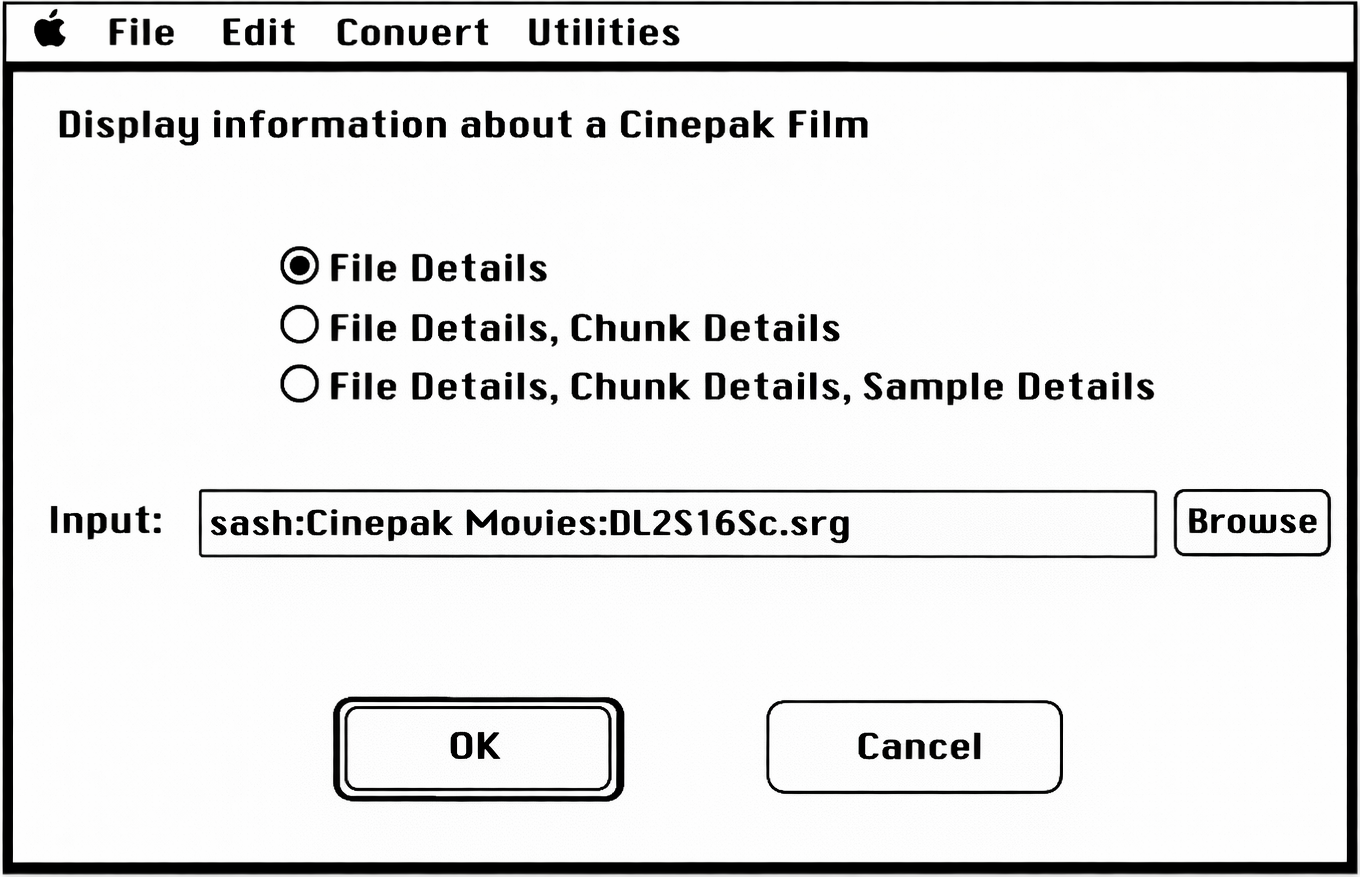
\includegraphics[width=0.7\textwidth]{figures/12/figure_8-g-restored.png}
\caption{\textit{Show Jaguar Cinepak Film Info} dialog}
\label{fig:show-cinepak-film-info-dialog}
\end{figure}
\FloatBarrier

To get just the basic information about a Jaguar Cinepak Film, select the \textit{File Details} radio button.
To also get the the details for each chunk of the Jaguar Cinepak Film, select the \textit{File Details, Chunk
Details} radio button. To get the maximum amount of information, including the details of each block
of sample data in the Jaguar Cinepak Film, select the radio button \textit{File Details, Chunk Details, Sample
Details}.

The specified film file will be analyzed and the requested information about the contents will be
dumped to the screen. To pause the screen output, hold down the mouse button, and release it when
you want to continue. (The information printed is identical to the FILMINFO tool available for MSDOS.)

\subsection{Show QuickTime Movie Info}

The \textit{ShowQuickTime Movie Info} menu item brings up a standard Macintosh File selector and allows
you to select a QuickTime movie. This will cause information about the movie, such as the movie
length, frame size, number of video frames per second, type of audio tracks, audio data format, and so
forth, will be printed into the console window.

\end{document}
